% CVPR 2023 Paper Template
% based on the CVPR template provided by Ming-Ming Cheng (https://github.com/MCG-NKU/CVPR_Template)
% modified and extended by Stefan Roth (stefan.roth@NOSPAMtu-darmstadt.de)

\documentclass[10pt,twocolumn,letterpaper]{article}

%%%%%%%%% PAPER TYPE  - PLEASE UPDATE FOR FINAL VERSION
% \usepackage[review]{cvpr}      % To produce the REVIEW version
% \usepackage{cvpr}              % To produce the CAMERA-READY version
\usepackage[pagenumbers]{cvpr} % To force page numbers, e.g. for an arXiv version

% Include other packages here, before hyperref.
\usepackage{graphicx}
\usepackage{amsmath}
\usepackage{amssymb}
\usepackage{booktabs}
\usepackage{color}
\usepackage{nicefrac}

\usepackage{etoolbox}
\makeatletter
\pretocmd{\chapter}{\addtocontents{toc}{\protect\addvspace{15\p@}}}{}{}
\pretocmd{\section}{\addtocontents{toc}{\protect\addvspace{5\p@}}}{}{}
\pretocmd{\subsection}{\addtocontents{toc}{\protect\addvspace{3\p@}}}{}{}
\makeatother
\usepackage{titletoc}

% new imported packages
\usepackage{xpatch}
\usepackage{array}
\usepackage{multirow}
\usepackage{graphicx}
\usepackage{xcolor,colortbl}
\usepackage{pifont}
\usepackage{enumitem}
\usepackage{xcolor}
\PassOptionsToPackage{dvipsnames}{xcolor}
\newcommand{\cmark}{\ding{51}}
\newcommand{\xmark}{\ding{55}}
\definecolor{Gray}{gray}{0.9}
\newcommand{\highlight}{\cellcolor{Gray}}
\definecolor{indian red}{RGB}{205,92,92}
% \newcommand{\algname}{\textbf{\textcolor{indian red}{UniAD}}\xspace}
\newcommand{\algname}{{{UniAD}}\xspace}
\usepackage{comment}
% \usepackage[accsupp]{axessibility}  % disabled: incompatible with XeLaTeX

\newcommand{\cl}[1]{\textcolor{magenta}{[CL]: #1}}
\newcommand{\HY}[1]{\textcolor{blue}{[HY]: #1}}
\newcommand{\yihan}[1]{\textcolor{green}{[yihan]: #1}}
\newcommand{\jz}[1]{\textcolor{cyan}{[JZ]: #1}}
% It is strongly recommended to use hyperref, especially for the review version.
% hyperref with option pagebackref eases the reviewers' job.
% Please disable hyperref *only* if you encounter grave issues, e.g. with the
% file validation for the camera-ready version.
%
% If you comment hyperref and then uncomment it, you should delete
% ReviewTempalte.aux before re-running LaTeX.
% (Or just hit 'q' on the first LaTeX run, let it finish, and you
%  should be clear).
\definecolor{mycitecolor}{rgb}{0, 0.4, 0.7}
\usepackage[pagebackref,breaklinks,colorlinks,bookmarks,citecolor=mycitecolor]{hyperref}


% Support for easy cross-referencing
\usepackage[capitalize]{cleveref}
\crefname{section}{Sec.}{Secs.}
\Crefname{section}{Section}{Sections}
\Crefname{table}{Table}{Tables}
\crefname{table}{Tab.}{Tabs.}

% Chinese support (v2)
\usepackage{xeCJK}
\setCJKmainfont{Noto Serif CJK SC}[ItalicFont=AR PL UKai TW MBE]
\setCJKsansfont{Noto Sans CJK SC}
\setCJKmonofont{Noto Sans CJK SC}
\raggedbottom
\renewcommand{\figurename}{图}
\renewcommand{\tablename}{表}
\renewcommand{\abstractname}{摘要}
\renewcommand{\refname}{参考文献}

%%%%%%%%% PAPER ID  - PLEASE UPDATE
\def\cvprPaperID{1655} % *** Enter the CVPR Paper ID here
\def\confName{CVPR}
\def\confYear{2023}


\begin{document}

%%%%%%%%% TITLE - PLEASE UPDATE
\title{
面向规划的自动驾驶
}


\author{
Yihan Hu$^{1,2\ast}$,
Jiazhi Yang$^{1\ast}$,
Li Chen$^{1\ast \dagger}$,
Keyu Li$^{1\ast}$,
Chonghao Sima$^1$,
Xizhou Zhu$^{3,1}$ \\
Siqi Chai$^2$,
Senyao Du$^2$,
Tianwei Lin$^2$,
Wenhai Wang$^1$,
Lewei Lu$^3$,
Xiaosong Jia$^{1}$ \\
Qiang Liu$^2$,
Jifeng Dai$^1$,
Yu Qiao$^1$,
Hongyang Li$^{1\dagger}$ \\
[2mm]
$^1$~OpenDriveLab and OpenGVLab, Shanghai AI Laboratory \\ 
$^2$~Wuhan University \quad
$^3$~SenseTime Research
\\ 
\normalsize{
$^\ast$Equal contribution \quad $^\dagger$Project lead}
\\
\normalsize{
\url{https://github.com/OpenDriveLab/UniAD}
}
}


\maketitle

%%%%%%%%% ABSTRACT

\begin{abstract}

现代自动驾驶系统被表征为按顺序排列的模块化任务，即感知、预测和规划。
%
为了执行多样化的任务并实现高级智能，现有方法要么为每个任务部署独立模型，要么设计具有独立子任务头的多任务范式。
%
然而，这些方法可能遭受累积误差或任务协调不足的问题。相反，本文认为，一个理想的框架应以最终目标——即自车的规划——为导向进行设计和优化。
%
基于这一方向，本文重新审视了感知和预测中的关键组件，并对各项任务进行优先级排序，使所有任务服务于规划。
%
本文提出了统一自动驾驶（UniAD（统一自动驾驶）），这是一个迄今为止最全面的框架，将全栈驾驶任务集成于单一网络中。
%
该框架精心设计以利用每个模块的优势，并从全局视角为智能体交互提供互补的特征抽象。各任务通过统一的查询（Query）接口进行通信，相互促进以服务于规划。
%
本文在具有挑战性的 nuScenes 基准上实例化了 UniAD（统一自动驾驶）。通过广泛的消融实验，这种设计理念的有效性得到了充分证明，在所有方面均显著优于之前的当前最优（SOTA）方法。代码和模型已公开。
\end{abstract}

%%%%%%%%% BODY TEXT
\section{引言}
\label{sec:intro}
\vspace{-4pt}
随着深度学习的成功发展，自动驾驶算法由一系列任务\footnote{在后续上下文中，本文会交替使用任务、模块、组件、单元和节点来表示特定任务（如检测）。}构成，
包括感知中的检测、跟踪、建图；以及预测中的运动预测和占用预测。
%
如\cref{fig:motivation}(a)所示，大多数工业解决方案为每个任务独立部署单独的模型~\cite{mobileye2022ces,nvidia2022drive}，只要车载芯片的资源带宽允许。
%
尽管这种设计简化了跨团队的研发难度，但由于优化目标的孤立性，它面临模块间信息丢失、误差累积和特征对齐不良的风险~\cite{luo2018faf,liang2020pnpnet,sadat2020p3}。


\begin{figure}[t!]
  \centering
  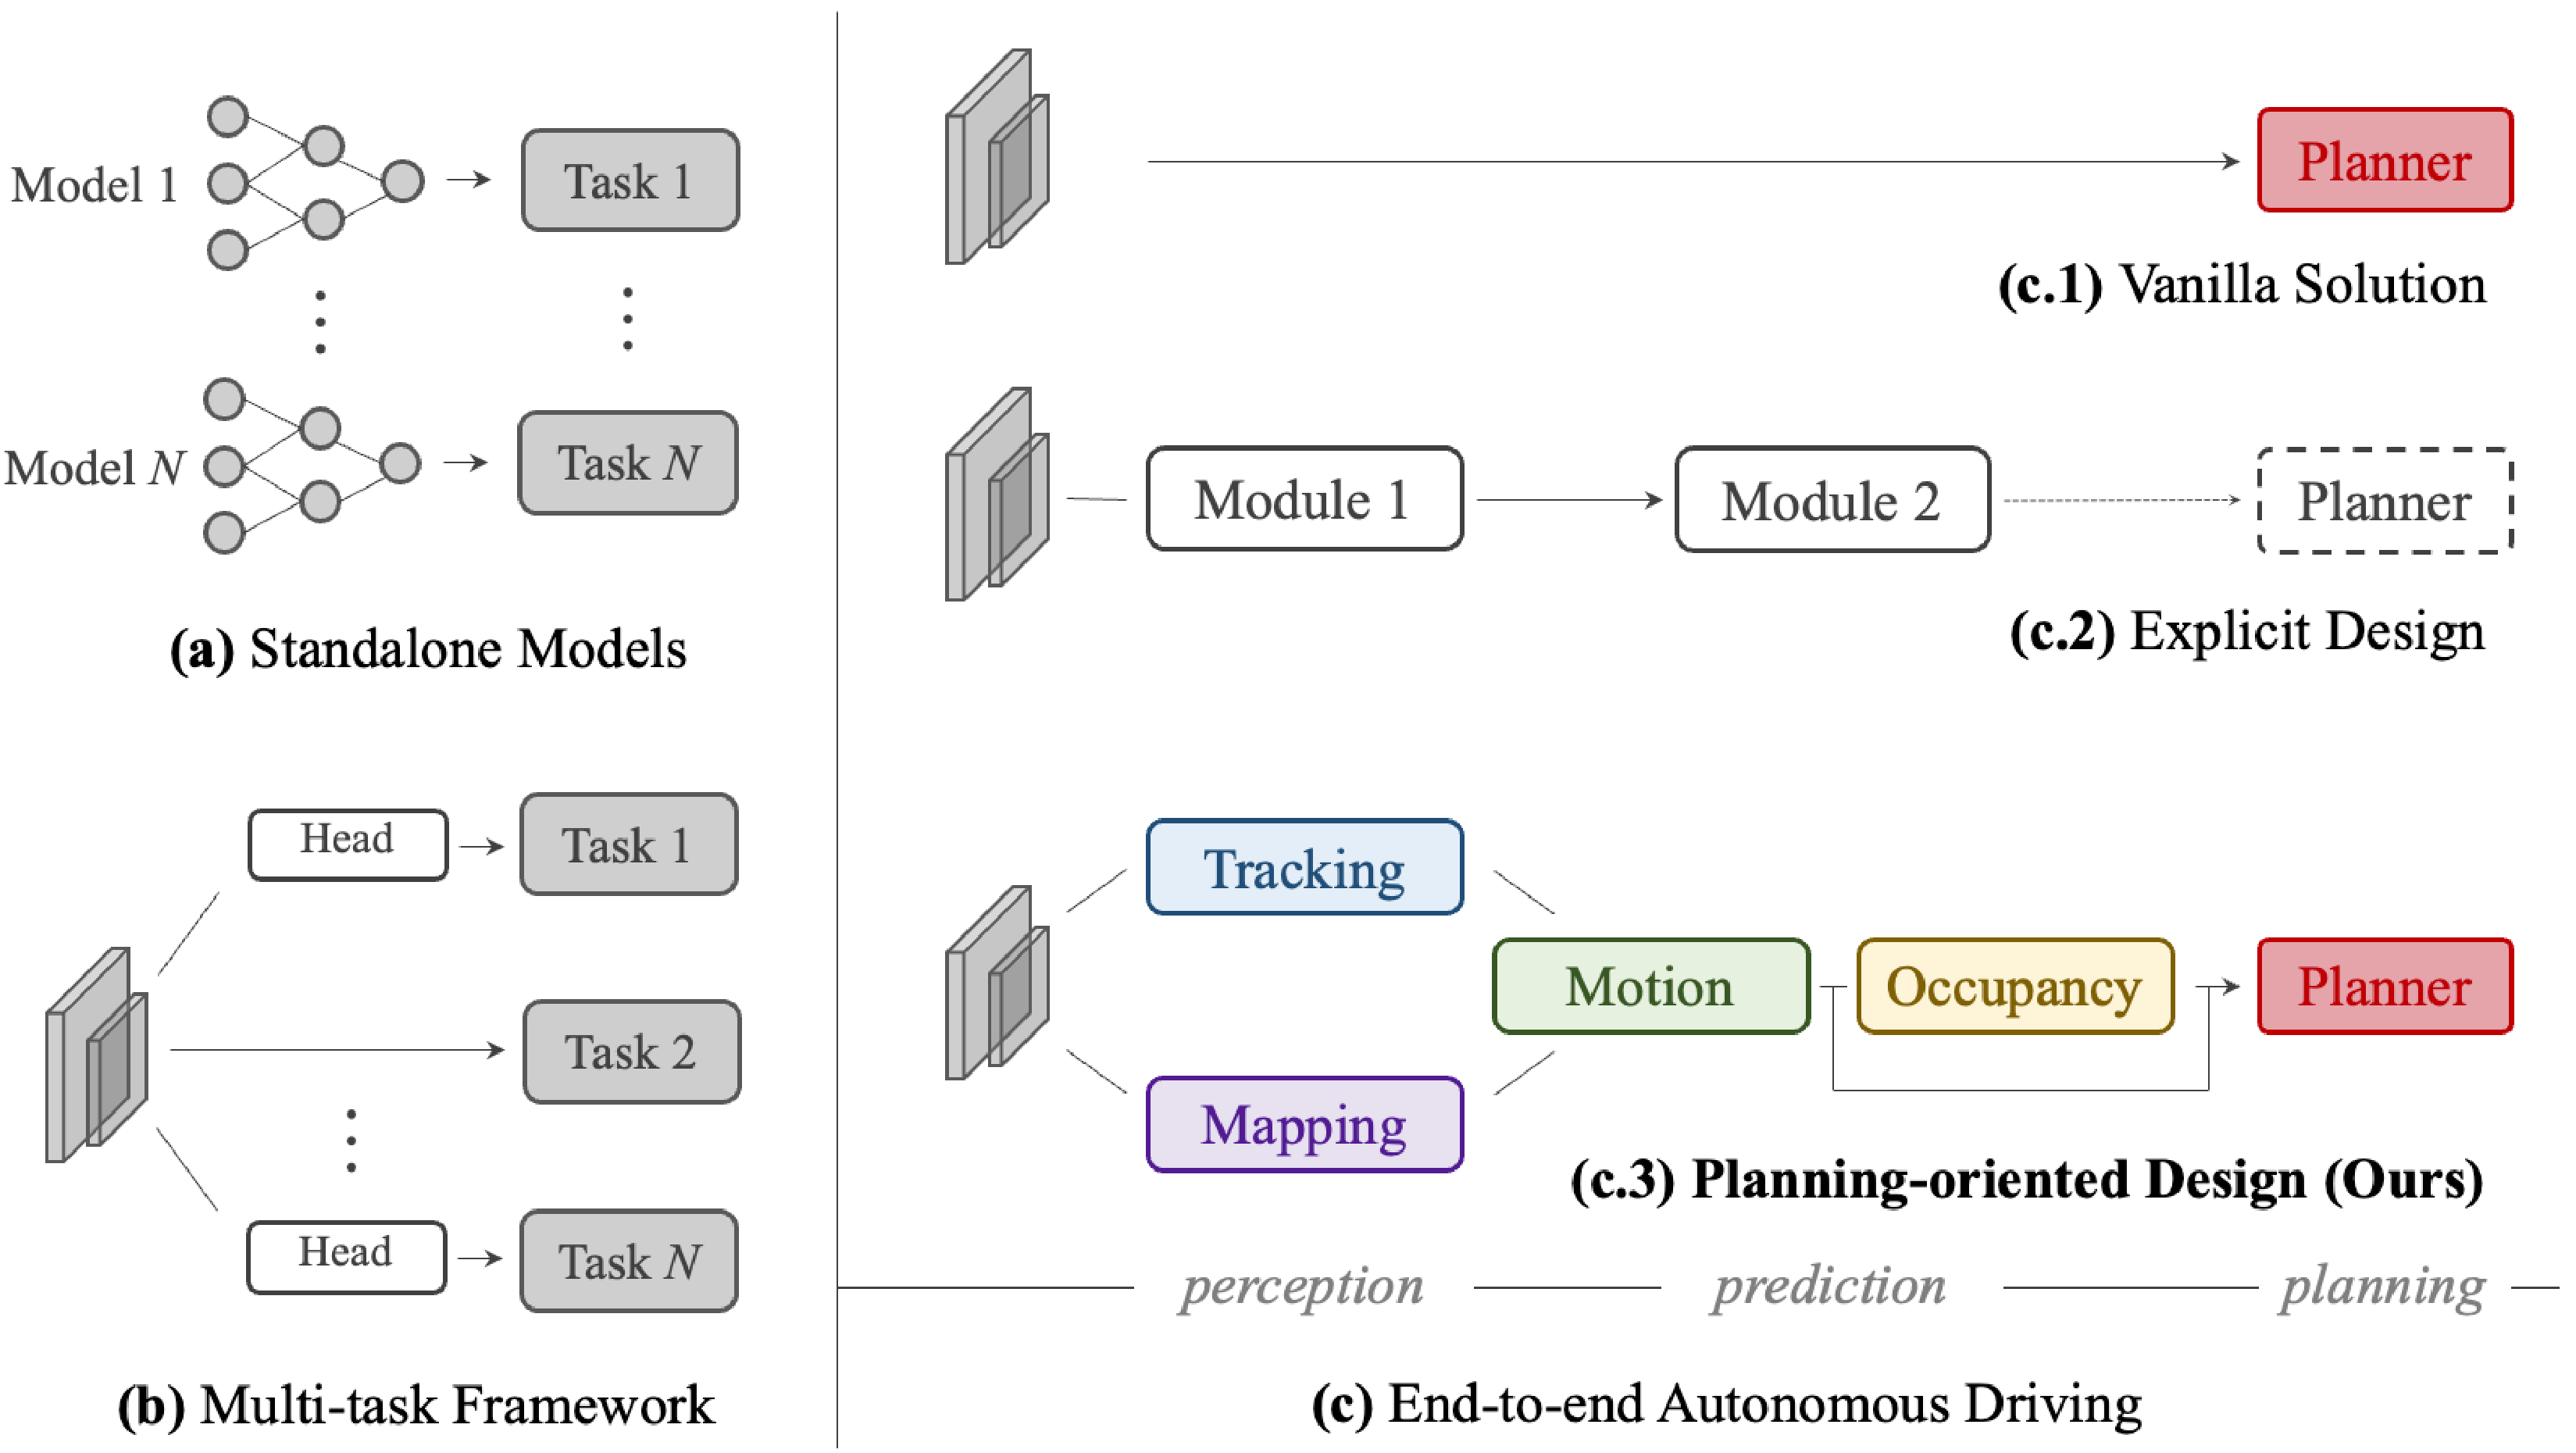
\includegraphics[width=\linewidth]{UniAD/figures/motivation.pdf}
  \vspace{-15pt}
  \caption{
  \textbf{自动驾驶框架的不同设计方案}对比。\textbf{(a)} 大多数工业解决方案为不同任务部署独立模型。\textbf{(b)} 多任务学习方案共享骨干网络，但使用分离的子任务头。
  %
  \textbf{(c)} 端到端范式将感知和预测中的模块统一。先前的尝试要么采用(c.1)中对规划的直接优化，要么在(c.2)中使用部分组件构建系统。相反，本文在(c.3)中认为，理想的系统应当{面向规划}，并合理组织前置任务以促进规划。
  }
  \label{fig:motivation}
  \vspace{-5pt}
\end{figure}




一种更优雅的设计是将广泛的任务整合到多任务学习（Multi-Task Learning，MTL）范式中，通过在共享特征提取器上添加多个特定任务的子任务头来实现，如\cref{fig:motivation}(b)所示。
%
这是许多领域的常见做法，包括通用视觉~\cite{wang2022ofa,zhu2022uniperceivermoe,reed2022gato}、自动驾驶\footnote{在本文中，自动驾驶中的多任务学习指的是\textit{超越}感知的任务。已有大量关于感知\textit{内部}多任务学习的工作，例如检测、深度、光流等。此类文献不在本文讨论范围内。}~\cite{zhang2022beverse,liang2022effective,zeng2019nmp,chen2022lav}，例如 Transfuser~\cite{Chitta2022transfuserpami}、BEVerse~\cite{zhang2022beverse} 以及工业化产品，如 Mobileye~\cite{mobileye2022ces}、Tesla~\cite{tesla2022aiday}、Nvidia~\cite{nvidia2022drive} 等。
%
在多任务学习中，跨任务的协同训练策略可以利用特征抽象；它可以轻松扩展到额外任务，并为车载芯片节省计算成本。
%
然而，这种方案可能导致不良的"负迁移"~\cite{crawshaw2020mtlsurvey, liu2022bevfusion}。


相比之下，端到端自动驾驶~\cite{chitta2021neat,wu2022tcp,chen2022lav,casas2021mp3,hu2022stp3} 的出现将感知、预测和规划中的所有节点统一为一个\textit{整体}。
%
前置任务的选择和优先级应以有利于规划为原则。
%
系统应当面向规划，精心设计包含特定组件，从而避免独立方案中的累积误差或多任务学习方案中的负迁移。\Cref{tab:motivation} 描述了不同框架设计的任务分类。

遵循端到端范式，一种"白板"做法是直接预测规划轨迹，而不使用任何感知和预测的显式监督，如\cref{fig:motivation}(c.1)所示。
%
开创性工作~\cite{chen2021wor,codevilla2018cil, codevilla2019cilrs, chen2020lbc, zhang2021roach, prakash2021transfuser, wu2022tcp, wu2023ppgeo} 在闭环仿真中验证了这种基础设计~\cite{Dosovitskiy17carla}。虽然这一方向值得进一步探索，但在安全性保障和可解释性方面仍显不足，尤其是在高度动态的城市场景中。
%
本文倾向于另一种视角，提出以下问题：
%
\emph{面向一个可靠且以规划为导向的自动驾驶系统，如何设计有利于规划的流水线？哪些前置任务是必需的？}

\begin{table}[t!]
    \centering
    \scalebox{0.7}{
	\begin{tabular}{l|l|ccc|cc|c}
		\toprule
		\multirow{2}{*}{设计} & \multirow{2}{*}{方法} & \multicolumn{3}{c|}{感知} & \multicolumn{2}{c|}{预测} & \multirow{2}{*}{规划} \\
		& & 检测 & 跟踪 & 建图 & 运动预测 & 占用 & \\
		\midrule
		\multirow{3}{*}{(b)} & NMP~\cite{zeng2019nmp} & \cmark & & & \cmark & & \cmark \\
		 & NEAT~\cite{chitta2021neat} &  &  & \cmark &  &  & \cmark \\
% 		 & Transfuser~\cite{Chitta2022transfuserpami} & \cmark &  & \cmark &  &  & \cmark \\
		 & BEVerse~\cite{zhang2022beverse} & \cmark & & \cmark & & \cmark & \\
		\midrule
		(c.1) & \cite{chen2021wor,chen2020lbc,prakash2021transfuser,wu2022tcp} &  &  &  & & & \cmark\\
		\midrule
		\multirow{6}{*}{(c.2)} & PnPNet$^\text{\textdagger}$~\cite{liang2020pnpnet} & \cmark & \cmark &  & \cmark & & \\
		 & ViP3D$^\text{\textdagger}$~\cite{gu2022vip3d} & \cmark & \cmark &  & \cmark & & \\
		 & P3~\cite{sadat2020p3} &  &  &  &  & \cmark & \cmark \\
		 & MP3~\cite{casas2021mp3} &  &  & \cmark &  & \cmark & \cmark \\
		 & ST-P3~\cite{hu2022stp3} &  &  & \cmark & & \cmark & \cmark \\
		 & LAV~\cite{chen2022lav} & \cmark &  & \cmark & \cmark &  & \cmark \\
		\midrule
		(c.3) & \textbf{\algname} (ours) & \cmark & \cmark & \cmark & \cmark & \cmark & \cmark \\
		\bottomrule
	\end{tabular}
	}
 \vspace{-5pt}
	\caption{\textbf{任务对比与分类。}``设计''列分类如\cref{fig:motivation}所示。``Det.''表示3D目标检测，``Map''表示在线建图，``Occ.''表示占用图预测。\textdagger: 这些工作并非直接为规划提出，但仍体现了联合感知与预测的精神。UniAD（统一自动驾驶）执行五项基本驾驶任务以促进规划。
 }
	\label{tab:motivation}
\end{table} 

一个直观的解决方案是显式地感知周围物体、预测未来行为并规划安全的驾驶操作，如\cref{fig:motivation}(c.2)所示。
%
现有方法~\cite{liang2020pnpnet, gu2022vip3d, sadat2020p3, casas2021mp3, hu2022stp3} 提供了很好的思路并取得了令人印象深刻的性能。然而，本文认为细节决定成败；先前的工作或多或少未能考虑某些组件（见\Cref{tab:motivation}中(c.2)块），偏离了面向规划的精神。
%
本文在补充材料中详细阐述了这些模块的定义、术语及其必要性。

为此，本文提出了\textbf{\algname}（统一自动驾驶），一个利用五项基本任务构建安全鲁棒系统的统一自动驾驶算法框架，如\cref{fig:motivation}(c.3)和\Cref{tab:motivation}(c.3)所示。
%
UniAD（统一自动驾驶）以面向规划的精神进行设计。本文强调这\textit{并非}简单的任务堆砌和工程工作。
%
关键组件是基于查询（Query）的设计来连接所有节点。与经典的边界框表示相比，查询具有更大的感受野，有助于缓解来自上游预测的累积误差。此外，查询可以灵活地建模和编码多种交互，例如多个智能体之间的关系。
%
据本文所知，UniAD（统一自动驾驶）是首个全面研究自动驾驶领域中感知、预测和规划等多种任务联合协作的工作。

本文的贡献总结如下：
%
\textbf{(a)} 本文遵循面向规划的哲学，提出了自动驾驶框架的新视角，并论证了有效任务协调的必要性，而非独立设计或简单的多任务学习。
%
\textbf{(b)} 本文提出了UniAD（统一自动驾驶），一个利用广泛任务的全面端到端系统。其关键设计是作为连接所有节点接口的查询设计。
%
由此，UniAD（统一自动驾驶）享有灵活的中间表示，并实现面向规划的多任务知识交换。
%
\textbf{(c)} 本文在具有挑战性的基准上针对真实场景实例化了UniAD（统一自动驾驶）。通过广泛的消融实验，本文验证了本文方法在所有方面均优于此前的当前最优（SOTA）方法。

\emph{本文希望这项研究能够为自动驾驶系统的目标驱动设计提供启发，为协调各种驾驶任务提供一个起点。}


\begin{figure*}[th!]
  \centering
  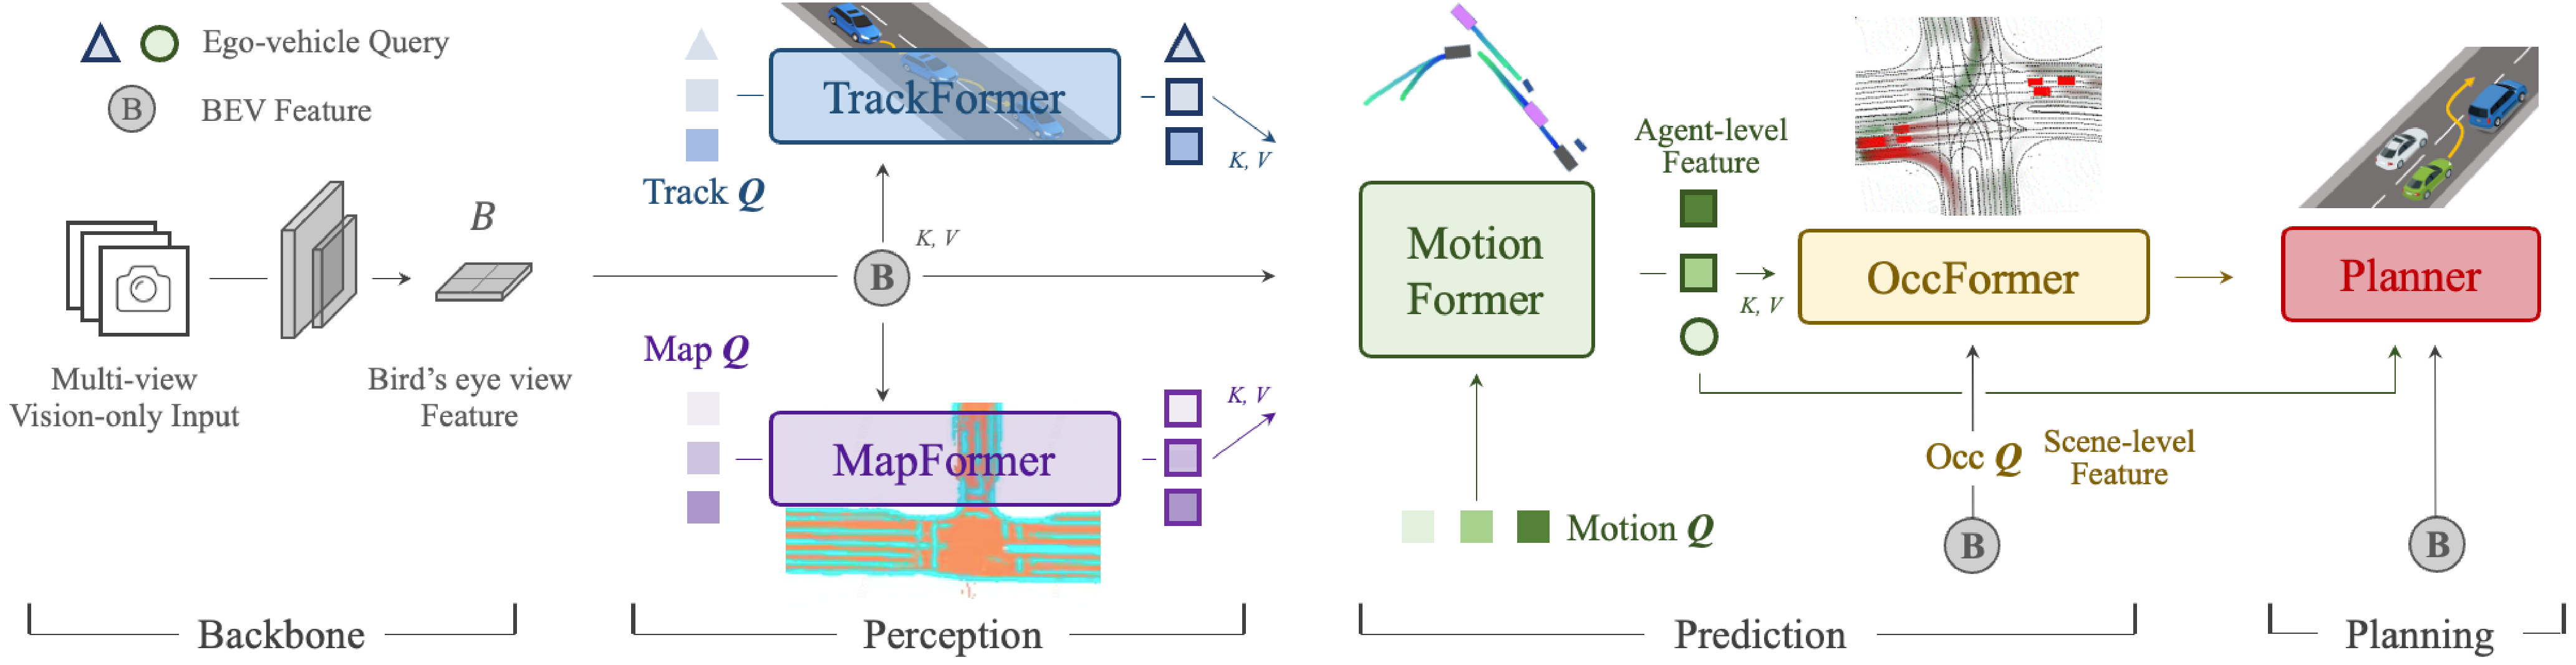
\includegraphics[width=\linewidth]{UniAD/figures/pipeline3_new.pdf}
  \vspace{-15pt}
  \caption{
  \textbf{流水线（Pipeline）} 统一自动驾驶（\algname）。本文遵循面向规划的哲学精心设计了该系统。不同于简单的任务堆叠，本文研究了感知和预测中每个模块的效果，利用从驾驶场景中的前置节点到最终规划的联合优化优势。
  %
  所有感知和预测模块采用Transformer解码器结构设计，以任务查询作为接口连接各个节点。
  %
  最后，一个简单的基于注意力的规划器利用从前置节点提取的知识预测自车的未来轨迹点。占用图仅用于可视化目的。
  }
  \label{fig:pipeline}
\end{figure*}


\section{方法}
\label{sec:method}
\vspace{-4pt}

\paragraph{概述.} 如\cref{fig:pipeline}所示，UniAD包含四个基于Transformer解码器的感知和预测模块以及一个最终的规划器。查询（Query）$Q$在整个流程中起到连接作用，用于建模驾驶场景中实体之间的不同交互。
%
具体而言，多相机图像序列被输入特征提取器，得到的透视图特征通过BEVFormer~\cite{li2022bevformer}中的现成BEV编码器转换为统一的鸟瞰视图（Bird's-Eye-View, BEV）特征$B$。需要注意的是，UniAD并不局限于特定的BEV编码器，研究者可以使用其他替代方案通过长期时序融合~\cite{han2023exploring, park2022solofusion}或多模态融合~\cite{liu2022bevfusion, liang2022bevfusion}提取更丰富的BEV表示。
%
在\textbf{TrackFormer}中，我们称之为跟踪查询（track queries）的可学习嵌入从$B$中查询智能体信息，以检测和跟踪智能体。
%
\textbf{MapFormer}将地图查询（map queries）作为道路元素（例如车道和分隔线）的语义抽象，并对地图执行全景分割。
%
利用上述表示智能体和地图的查询，\textbf{MotionFormer}捕获智能体与地图之间的交互并预测每个智能体的未来轨迹。
%
由于每个智能体的行为会显著影响场景中的其他智能体，该模块对所有考虑的智能体进行联合预测。
%
同时，本文设计了自车查询来显式建模自车，使其能够在以场景为中心的范式中与其他智能体进行交互。
%
\textbf{OccFormer}以BEV特征$B$作为查询，配备以智能体维度的知识作为键和值，预测保留智能体身份的多步未来占用状态。
%
最后，\textbf{规划器}利用来自MotionFormer的富有表现力的自车查询预测规划结果，并使其远离OccFormer预测的占用区域以避免碰撞。


\subsection{感知：跟踪与建图}
\vspace{-4pt}
\paragraph{TrackFormer.} 该模块联合执行检测和多目标跟踪（Multi-Object Tracking, MOT），无需不可微的后处理。受~\cite{zeng2021motr, zhang2022mutr3d}启发，本文采用了类似的查询设计。
%
除目标检测~\cite{carion2020detr, zhu2020deformabledetr}中使用的常规检测查询（detection queries）外，还引入了额外的跟踪查询（track queries）用于跨帧跟踪智能体。
%
具体而言，在每个时间步，初始化的检测查询负责检测首次感知到的新生智能体，而跟踪查询则持续建模先前帧已检测到的智能体。检测查询和跟踪查询均通过关注BEV特征$B$来捕获智能体抽象表示。
%
随着场景不断变化，当前帧的跟踪查询通过自注意力模块与先前记录的跟踪查询交互，以聚合时序信息，直到对应智能体完全消失（在一定时间内未被跟踪）。
%
与~\cite{carion2020detr}类似，TrackFormer包含$N$层，最终输出状态$Q_A$为下游预测任务提供$N_a$个有效智能体的知识。
%
除编码自车周围其他智能体的查询外，本文在查询集中引入一个特殊的\textit{自车查询}以显式建模自车，该查询进一步用于规划。


\paragraph{MapFormer.} 本文基于2D全景分割方法Panoptic SegFormer~\cite{li2022panopticseg}设计了该模块。
%
本文将道路元素稀疏地表示为地图查询（map queries），以帮助下游运动预测，其中编码了位置和结构知识。针对驾驶场景，本文将车道、分隔线和人行横道设为前景事物（things），将可行驶区域设为背景内容（stuff）~\cite{kirillov2019panoptic}。
%
MapFormer也具有$N$个堆叠层，每层输出结果都受到监督，而仅最后一层更新的查询$Q_M$被传递至MotionFormer进行智能体-地图交互。


\subsection{预测：运动预测}
\label{sec:motion-method}
\vspace{-4pt}
近期研究已证明Transformer结构在运动任务上的有效性~\cite{liu2021multimodal, yuan2021agentformer, jia2021allocentric, jia2022hdgt, nayakanti2022wayformer, shi2022motiontransformer, ngiam2021scenetransformer}，受此启发，本文在端到端设置中提出了MotionFormer。
%
利用来自TrackFormer和MapFormer的高度抽象的动态智能体查询$Q_A$和静态地图查询$Q_M$，MotionFormer以场景为中心的方式预测所有智能体的多模态未来运动，即top-$k$条可能的轨迹。
%
该范式通过单次前向传播生成帧中所有智能体的轨迹，极大节省了将整个场景对齐到每个智能体坐标系的计算成本~\cite{kim2022stopnet}。
%
同时，本文将通过MotionFormer传递来自TrackFormer的\textit{自车查询}，使自车在考虑未来动态的情况下与其他智能体进行交互。
%
形式上，运动输出表示为
$\!\{\hat{\mathbf{x}}_{i,k}\!\in\!\mathbb{R}^{T\!\times\!2} | i\!=1,\dots,N_a; k\!=\!1,\dots,\mathcal{K}\}$
，其中$i$索引智能体，$k$索引轨迹模态，$T$为预测时间范围的长度。

\paragraph{MotionFormer.} 它由$N$层组成，每层捕获三种类型的交互：智能体-智能体、智能体-地图和智能体-目标点。
%
对于每个运动查询$Q_{i,k}$（稍后定义，为简洁起见下文省略下标$i$、$k$），其与其他智能体$Q_{A}$或地图元素$Q_{M}$的交互可表示为：
%
\begin{equation}
\label{eq:agent-agent}
    Q_{a/m} = \texttt{MHCA}(\texttt{MHSA}(Q), Q_A/Q_M),
\end{equation}
%
其中$\texttt{MHCA}$、$\texttt{MHSA}$分别表示多头交叉注意力（Multi-Head Cross-Attention）和多头自注意力（Multi-Head Self-Attention）~\cite{vaswani2017transformer}。
%
由于关注目标位置（即目标点）对精炼预测轨迹也很重要，本文通过可变形注意力~\cite{zhu2020deformabledetr}设计了智能体-目标点注意力，如下所示：
\begin{equation}
\label{eq:agent-bev}
    Q_{g} = \texttt{DeformAttn}(Q, \hat{\mathbf{x}}_{T}^{l-1}, B),
\end{equation}
其中$\hat{\mathbf{x}}_T^{l-1}$是前一层的预测轨迹端点。$\texttt{DeformAttn}(q,\!r,\!x)$是一个可变形注意力模块，接收查询$q$、参考点$r$和空间特征$x$。
%
它围绕参考点对空间特征执行稀疏注意力。通过这种方式，预测轨迹因感知到端点周围环境而进一步精炼。
%
所有三种交互并行建模，生成的$Q_a$、$Q_m$和$Q_g$被拼接并传入多层感知机（MLP），得到查询上下文$Q_{\text{ctx}}$。随后，$Q_{\text{ctx}}$被送入下一层进行精炼，或在最后一层解码为预测结果。
%
\paragraph{运动查询（Motion queries）.} MotionFormer每层的输入查询称为运动查询（motion queries），包含两个部分：前一层产生的查询上下文$Q_{\text{ctx}}$（如前所述）和查询位置$Q_{\text{pos}}$。
%
具体而言，$Q_{\text{pos}}$以四种方式整合位置知识，如\cref{eq:qpos}所示：(1) 场景级锚点$I^s$的位置；(2) 智能体级锚点$I^a$的位置；(3) 智能体$i$的当前位置；(4) 预测的目标点。
%
\begin{equation}
\label{eq:qpos}
\begin{aligned}
    Q_{\text{pos}} =\ &\text{MLP}(\text{PE}(I^s))  + \text{MLP}(\text{PE}(I^a))  \\
    +\ &\text{MLP}(\text{PE}(\hat{\mathbf{x}}_0)) + \text{MLP}(\text{PE}(\hat{\mathbf{x}}_T^{l-1})).
\end{aligned}
\end{equation}
此处利用正弦位置编码$\text{PE}(\cdot)$后接MLP来编码位置点，在第一层中将$\hat{\mathbf{x}}_T^0$设为$I^s$（同样省略了下标$i,k$）。
%
场景级锚点表示全局视角下的先验运动统计信息，而智能体级锚点捕获局部坐标系中的可能意图。两者均通过对真实轨迹的端点执行k-means算法聚类得到，以缩小预测的不确定性。
%
与先验知识不同，起始点为每个智能体提供定制的位置嵌入，预测端点则作为动态锚点，以从粗到细的方式逐层优化。


\paragraph{非线性优化（Non-linear Optimization）.}
与能够直接访问真实感知结果（即智能体位置和对应轨迹）的传统运动预测工作不同，本文在端到端范式中考虑了来自前置模块的预测不确定性。
%
从不够精确的检测位置或航向角直接回归真实轨迹点可能导致预测轨迹出现过大曲率和加速度的不合理结果。
%
为解决此问题，本文采用非线性平滑器~\cite{nuplan}来调整目标轨迹，使其在上游模块预测的不精确起始点下仍具有物理可行性。该过程如下：
\begin{equation}
\label{eq:non-linear-argmin}
    \tilde{\mathbf{x}}^* = \arg \min _{\mathbf{x}} c(\mathbf{x}, \tilde{\mathbf{x}} ),
\end{equation}
%
其中$\tilde{\mathbf{x}}$和$\tilde{\mathbf{x}}^*$分别表示真实轨迹和平滑后的轨迹，$\mathbf{x}$通过多帧打靶法（multiple-shooting）~\cite{bock1984multiple}生成，代价函数如下：
%
\begin{equation}
\label{eq:non-linear-cost}
% \begin{aligned}
    c(\mathbf{x}, \tilde{\mathbf{x}} ) = \lambda_{\text{xy}} \lVert\mathbf{x}, \tilde{\mathbf{x}}\rVert_2 +  \lambda_{\text{goal}} \lVert\mathbf{x}_{T}, \tilde{\mathbf{x}}_{T}\rVert_2
    +  \sum_{\phi\in \Phi} \phi(\mathbf{x}),
\end{equation}
其中$\lambda_{\text{xy}}$和$\lambda_{\text{goal}}$为超参数，运动学函数集$\Phi$包含五个项：加加速度（jerk）、曲率、曲率变化率、加速度和横向加速度。该代价函数约束目标轨迹遵循运动学约束。此目标轨迹优化仅在训练中进行，不影响推理。



\subsection{预测：占用预测}
\label{sec:occ-method}
\vspace{-4pt}

占用网格图（Occupancy grid map）是一种离散化的BEV表示，其中每个单元格包含是否被占用的置信度，占用预测任务旨在发现网格图未来的变化。
%
先前的方法利用RNN结构从观测到的BEV特征中随时间展开未来预测~\cite{hu2021fiery, hu2022stp3, zhang2022beverse}。
%
然而，这些方法严重依赖高度手工设计的聚类后处理来生成每个智能体的占用图，因为它们大多通过将BEV特征整体压缩到RNN隐藏状态中，忽略了智能体的身份信息。
%
由于缺乏对智能体级别知识的有效利用，它们难以全局预测所有智能体的行为，而这对于理解场景演变至关重要。
%
为解决这一问题，本文提出了OccFormer，从两个方面融合场景级和智能体级语义：(1) 密集型场景特征在展开到未来时间范围时，通过精心设计的注意力模块获取智能体级别特征；(2) 通过智能体级别特征与密集型场景特征之间的矩阵乘法轻松生成实例级占用，无需繁琐的后处理。

OccFormer由$T_o$个顺序块组成，其中$T_o$表示预测时间范围。需要注意的是，由于密集型占用的计算成本较高，$T_o$通常小于运动任务中的$T$。
%
每个块接收来自前一层的丰富智能体特征$G^t$和状态（密集特征）$F^{t-1}$作为输入，并生成时间步$t$的$F^t$，同时考虑实例级和场景级信息。
%
为获取包含动态和空间先验的智能体特征$G^t$，
本文将MotionFormer的运动查询在模态维度上进行最大池化，记为$Q_X\!\in\!\mathbb{R}^{N_a\!\times\!D}$，其中$D$为特征维度。然后通过时序特定的MLP将其与上游的跟踪查询$Q_{A}$和当前位置嵌入$P_{A}$融合：
%
\begin{equation}
\label{eq:query fuse}
    G^t = \text{MLP}_{t}([Q_{A}, P_{A}, Q_{X}]),\ t={1,\dots,T_o},
\end{equation}
%
其中$[\cdot]$表示拼接。对于场景级知识，BEV特征$B$被降采样到\nicefrac{1}{4}分辨率以提高训练效率，作为第一个块的输入$F^0$。
%
为进一步节省训练内存，每个块采用下采样-上采样的方式，中间使用注意力模块在\nicefrac{1}{8}下采样特征上执行像素-智能体交互，该特征记为$F_{\text{ds}}^t$。

\vspace{-7pt}
\paragraph{像素-智能体交互（Pixel-agent interaction）} 旨在统一预测未来占用时的场景级和智能体级理解。
%
本文将密集特征$F_\text{ds}^t$作为查询，实例级特征作为键和值，以随时间更新密集特征。具体而言，$F^t_{\text{ds}}$首先经过自注意力层建模远距离网格之间的响应，然后通过交叉注意力层建模智能体特征${G^{t}}$与每个网格特征之间的交互。
%
此外，为对齐像素-智能体的对应关系，本文通过注意力掩码约束交叉注意力，限制每个像素仅关注在时间步$t$占据它的智能体，受~\cite{cheng2021mask2former}启发。
%
密集特征的更新过程表示为：
\begin{equation}
\label{eq:mask attention}
    D_{\text{ds}}^t = \texttt{MHCA}( \texttt{MHSA}(F_{\text{ds}}^t), G^t, \text{attn\_mask} = O_m^t).
\end{equation}
注意力掩码$O_m^t$在语义上类似于占用图，通过将额外的智能体级特征与密集特征$F_{\text{ds}}^t$相乘生成，该智能体级特征称为掩码特征$M^t=\text{MLP}({G^{t}})$。
%
经过\cref{eq:mask attention}中的交互过程后，$D_{\text{ds}}^t$上采样到$B$的\nicefrac{1}{4}大小。本文将$D_{\text{ds}}^t$与块输入$F^{t-1}$相加作为残差连接，所得特征$F^t$传递至下一个块。

\vspace{-7pt}
\paragraph{实例级占用（Instance-level occupancy）.} 该表示保留了每个智能体身份的占用信息。可以通过矩阵乘法简单获得，类似于近期基于查询的分割工作~\cite{cheng2021maskformer, li2022maskdino}。
%
形式上，为获得BEV特征$B$原始大小$H\!\times\!W$的占用预测，场景级特征$F^t$通过卷积解码器上采样到$F_{\text{dec}}^t\!\in\!\mathbb{R}^{C\!\times\!H\!\times\!W}$，其中$C$为通道维度。
%
对于智能体级特征，本文通过另一个MLP将粗略的掩码特征$M^t$进一步更新为占用特征$U^t\!\in\!\mathbb{R}^{N_a\!\times\!C}$。实验发现，从掩码特征$M^t$而非原始智能体特征${G^{t}}$生成$U^t$可获得更优性能。
%
时间步$t$的最终实例级占用为：
\begin{equation}
    \hat{O}_A^t = U^t \cdot F_{\text{dec}}^t.
\end{equation}


\subsection{规划}
\label{sec:method-plan}
\vspace{-4pt}
在没有高精地图（High-Definition Map, HD Map）或预定义路线的情况下，规划通常需要高级指令来指示行驶方向~\cite{casas2021mp3, hu2022stp3}。
%
遵循这一思路，本文将原始导航信号（即左转、右转和直行）转换为三个可学习的嵌入向量，称为指令嵌入（command embeddings）。
%
由于来自MotionFormer的自车查询已表达其多模态意图，本文为其配备指令嵌入以形成"规划查询（plan query）"。规划查询关注BEV特征$B$以感知周围环境，然后解码为未来轨迹点$\hat{\tau}$。

为进一步避免碰撞，本文仅在推理阶段基于牛顿法优化$\hat{\tau}$，如下所示：
\begin{equation}
\label{eq:plan-argmin}
    \tau^* = \arg \min _{\tau} f(\tau, \hat{\tau}, \hat{O} ),
\end{equation}
其中$\hat{\tau}$为原始规划预测，$\tau^*$表示优化后的规划结果，通过从多帧打靶法（multiple-shooting）\cite{bock1984multiple}生成的轨迹$\tau$中选择使代价函数$f(\cdot)$最小的轨迹得到。$\hat{O}$是由OccFormer的实例级占用预测合并而成的经典二值占用图。代价函数$f(\cdot)$计算如下：
%
\begin{equation}
\label{eq:col-cost}
    f(\tau, \hat{\tau}, \hat{O} ) = \lambda_{\text{coord}}  \lVert\tau, \hat{\tau}\rVert_2 +
    \lambda_{\text{obs}}  \sum_{t} \mathcal{D}(\tau_{t}, \hat{O}^{t}),
\end{equation}
\vspace{-10pt}
\begin{equation}
\label{eq:col-dist}
    \mathcal{D}(\tau_{t}, \hat{O}^{t}) = \sum_{(x, y) \in \mathcal{S}}
    \frac{1}{\sigma \sqrt{2\pi}}
    \text{exp} (-\frac{\lVert \tau_{t} - (x, y) \rVert_2^2}{2\sigma^2}).
\end{equation}
%
其中$\lambda_{\text{coord}}$、$\lambda_{\text{obs}}$和$\sigma$为超参数，$t$索引未来时间范围中的时间步。$l_2$代价将轨迹拉向原始预测结果，而碰撞项$\mathcal{D}$将其推离占用网格，考虑的周围位置限制在$ \mathcal{S}=\{(x, y) | \lVert(x, y) - \tau_t\rVert_{2} < d, \hat{O}_{x, y}^t = 1\}$内。

\begin{table*}[t!]
    \definecolor{Gray}{gray}{0.9}
	\begin{center}
		\resizebox{\textwidth}{!}{
			\begin{tabular}{l|ccccc|ccc|cc|ccc|cccc|cc}
				\toprule
				\multirow{2}{*}{ID} &
				\multicolumn{5}{c|}{Modules} & 
				\multicolumn{3}{c|}{Tracking} & 
				\multicolumn{2}{c|}{Mapping} & 
				\multicolumn{3}{c|}{Motion Forecasting} & 
				\multicolumn{4}{c|}{Occupancy Prediction} & \multicolumn{2}{c}{Planning}  \\
				& Track & Map & Motion & Occ. & Plan& AMOTA$\uparrow$ & AMOTP$\downarrow$ &IDS$\downarrow$ & IoU-lane$\uparrow$ & IoU-road$\uparrow$ & minADE$\downarrow$ & minFDE$\downarrow$ & MR$\downarrow$ & IoU-n.$\uparrow$& IoU-f.$\uparrow$ & VPQ-n.$\uparrow$ & VPQ-f.$\uparrow$& avg.L2$\downarrow$  & avg.Col.$\downarrow$   \\
				\midrule
				0$^\ast$ & \cmark & \cmark & \cmark & \cmark & \cmark & 0.356 & 1.328 &893  & 0.302 & 0.675 & 0.858 & 1.270 & 0.186 & 55.9 & 34.6 & 47.8 &26.4  & 1.154 & 0.941 \\
				\midrule
				1 & \cmark & & & & & \highlight{0.348} & \highlight{1.333} & \highlight{791} & \highlight{-} & \highlight{-} & - & - & - & - & - & - & - & - & - \\
				2 & & \cmark & & & & \highlight{-} & \highlight{-} & \highlight{-} & \highlight{\textbf{0.305}} & \highlight{\underline{0.674}} & - & - & - & - & - & - & - & - & - \\
				3 & \cmark & \cmark & & & & \highlight{0.355} & \highlight{1.336} & \highlight{\underline{785}} & \highlight{0.301} & \highlight{0.671} & - & - & - & - & - & - & - & - & - \\
				\midrule
				4 &  &  & \cmark &  &  & - & - & - & - & - & \highlight{0.815} & \highlight{1.224} & \highlight{0.182} & - & - & - & - & - & - \\
				5 & \cmark &  & \cmark &  &  & \underline{0.360} & 1.350 & 919 & - & - & \highlight{0.751} & \highlight{1.109} & \highlight{0.162} & - & - & - & - & - & - \\
				6 & \cmark & \cmark & \cmark &  &  & 0.354 & 1.339 & 820 & 0.303 & 0.672 & \highlight{0.736(-9.7\%)} & \highlight{1.066(-12.9\%)} & \highlight{0.158} & - & - & - & - & - & - \\
				\midrule
				7 &  &  &  & \cmark &  & - & - & - & - & - & \highlight{-} & \highlight{-} & \highlight{-} & \highlight{60.5}& \highlight{37.0}& \highlight{52.4}	&\highlight{29.8}  & - & - \\
				8 & \cmark &  &  & \cmark &  & \underline{0.360} & \textbf{1.322} & 809 & - & - & \highlight{-} & \highlight{-} & \highlight{-} & \highlight{\underline{62.1}} & \highlight{38.4} & \highlight{52.2} & \highlight{32.1}  & - & - \\
				9 & \cmark & \cmark & \cmark & \cmark & & 0.359 & 1.359 & 1057 & \underline{0.304} & \textbf{0.675} & \highlight{\textbf{0.710}(-3.5\%)} & \highlight{\textbf{1.005}(-5.8\%)} & \highlight{\textbf{0.146}} &\highlight{\textbf{62.3}} & \highlight{\underline{39.4}} & \highlight{\textbf{53.1}} & \highlight{\underline{32.2}} & - & - \\
				\midrule
				10 &  &  &  &  & \cmark &  & - & - & - & - & - & - & - & - & - & - & - & \highlight{1.131} & \highlight{0.773} \\
				11 & \cmark & \cmark & \cmark &  & \cmark &  \textbf{0.366} & 1.337 & 889 & 0.303 & 0.672 & 0.741 & 1.077 & 0.157&  - & - & - & - & \highlight{\underline{1.014}} & \highlight{\underline{0.717}} \\
				12 & \cmark & \cmark & \cmark & \cmark & \cmark & 0.358	 & \underline{1.334} & \textbf{641} & 0.302 & 0.672 & \underline{0.728} & \underline{1.054} & \underline{0.154} & \textbf{62.3} & \textbf{39.5} & \underline{52.8} & \textbf{32.3} & \highlight{\textbf{1.004}} & \highlight{\textbf{0.430}} \\
				\bottomrule
			\end{tabular}
		}
	\end{center}
 \vspace{-15pt}
	\caption{\textbf{各任务有效性的详细消融实验。} 可以看出两个感知子任务极大帮助了运动预测，同时预测性能也受益于两个预测模块的统一。借助所有前置表示，本文以规划为导向的设计显著提升了安全性。
 %
 \algname{}在预测和规划任务上大幅优于朴素MTL方案，并且具有\textit{无显著感知性能下降}的优势。为简洁起见，仅展示主要指标。  
 ``avg.L2''和``avg.Col''是规划时间范围内的平均值。$\ast$: ID-0是为每个任务设置独立子任务头的MTL方案。
 }
	\label{tab:abl-module}
\end{table*} 



\subsection{学习}
\vspace{-4pt}

\algname{}采用两阶段训练。首先联合训练感知部分（即跟踪和建图模块）数个周期（实验中为6个周期），然后端到端训练所有感知、预测和规划模块共20个周期。实验发现两阶段训练更加稳定。各损失函数的详细内容请参见补充材料。

\vspace{-4pt}
\paragraph{共享匹配（Shared matching）.} 由于UniAD涉及实例级建模，需要在感知和预测任务中将预测与真实值集合进行配对。
%
与DETR~\cite{carion2020detr,li2022panopticseg}类似，在跟踪和在线建图阶段采用了二分图匹配算法。对于跟踪而言，来自检测查询的候选框与新出现的真实目标进行配对，而来自跟踪查询的预测则继承前一帧的分配结果。
%
跟踪模块中的匹配结果在运动和占用节点中被重用，以在端到端框架中从历史轨迹到未来运动一致地建模智能体。


\section{实验}
\label{sec:experiments}
\vspace{-4pt}

本文在具有挑战性的nuScenes数据集~\cite{caesar2020nuscenes}上进行实验。在本节中，我们从三个方面验证本文设计的有效性：揭示任务协调优势及其对规划影响的联合分析结果、各任务与先前方法的模块化对比结果，以及特定模块设计空间的消融实验。由于篇幅限制，完整的实验协议、部分消融实验和可视化结果详见补充材料。

\subsection{联合结果}
\label{sec:exp-joint}
\vspace{-4pt}
本文进行了广泛的消融实验，如\Cref{tab:abl-module}所示，以证明端到端流程中前置任务的有效性和必要性。该表每一行显示了在纳入第二列\textit{模块}中列出的任务模块时的模型性能。
第一行（ID-0）作为具有独立子任务头的朴素多任务基线供对比。
每个指标的最佳结果以粗体标记，次优结果以加下划线标记。

\vspace{-4pt}
\paragraph{安全规划的路线图。}
由于预测比感知更接近规划，
本文首先研究框架中的两类预测任务，即运动预测和占用预测。在Exp.10-12中，仅当同时引入两个任务时（Exp.12），规划L2和碰撞率两个指标均达到最佳结果，优于没有任何中间任务的朴素端到端规划（Exp.10, \cref{fig:motivation}(c.1)）。
%
因此本文得出结论，安全规划目标需要这两类预测任务。
%
进一步，Exp.7-9展示了两类预测的协同效应。当它们紧密集成时，两个任务的性能均得到提升（Exp.9, minADE降低3.5\%，minFDE降低5.8\%，MR降低1.3个百分点，IoU-f.提高2.4个百分点，VPQ-f.提高2.4个百分点），证明了同时包含智能体表示和场景表示的必要性。
%
同时，为实现更优的运动预测性能，本文在Exp.4-6中探索感知模块的贡献。值得注意的是，同时纳入跟踪和建图模块为预测结果带来了显著提升（minADE降低9.7\%，minFDE降低12.9\%，MR降低2.3个百分点）。
%
Exp.1-3表明，同时训练感知子任务可获得与单任务相当的性能。
%
此外，与朴素多任务学习（Exp.0, \cref{fig:motivation}(b)）相比，Exp.12在所有关键指标上显著领先（minADE降低15.2\%，minFDE降低17.0\%，MR降低3.2个百分点，IoU-f.提高4.9个百分点，VPQ-f.提高5.9个百分点，avg.L2降低0.15m，avg.Col.降低0.51个百分点），展示了本文以规划为导向的设计的优越性。


\subsection{模块化结果}
\label{sec:exp-sota}
\vspace{-4pt}
遵循感知-预测-规划的顺序，本文在nuScenes验证集上报告每个任务模块与先前当前最优方法的性能对比。需要注意的是，UniAD通过单一训练网络联合执行所有这些任务。每个任务的主要指标在表中以灰色背景标记。

\vspace{-6pt}
\paragraph{感知结果.} 在\Cref{tab:sota-track}中的多目标跟踪方面，与MUTR3D~\cite{zhang2022mutr3d}和ViP3D~\cite{gu2022vip3d}相比，UniAD的AMOTA(\%)分别提升了\textbf{+6.5}和\textbf{+14.2}。
%
此外，UniAD取得了最低的ID切换分数，展示了每个轨迹段的时间一致性。对于\Cref{tab:sota-map}中的在线建图，UniAD在车道分割（与BEVFormer相比IoU(\%)提升\textbf{+7.4}）方面表现良好，这对于运动模块中下游的智能体-道路交互至关重要。
%
由于本文的跟踪模块采用端到端范式，其仍然逊于具有复杂关联机制的检测后跟踪方法（如Immortal Tracker~\cite{wang2021immortal}），并且建图结果在特定类别上落后于先前以感知为导向的方法。本文认为UniAD旨在利用感知信息使\textit{最终}规划受益，而非以全部模型能力优化感知。

\vspace{-6pt}
\paragraph{预测结果.} \Cref{tab:sota-motion}展示了运动预测结果，UniAD显著优于先前基于视觉的端到端方法。与PnPNet-vision~\cite{liang2020pnpnet}和ViP3D~\cite{gu2022vip3d}相比，minADE上的预测误差分别降低了\textbf{38.3\%}和\textbf{65.4\%}。
%
在\Cref{tab:sota-occ}报告的占用预测方面，UniAD在近处区域取得了显著进展，与带有大量数据增强的FIERY~\cite{hu2021fiery}和BEVerse~\cite{zhang2022beverse}相比，IoU-near(\%)分别提升\textbf{+4.0}和\textbf{+2.0}。

\vspace{-6pt}
\paragraph{规划结果.} 得益于自车查询和占用中的丰富时空信息，与ST-P3~\cite{hu2022stp3}相比，UniAD在规划时间范围内的平均L2误差和碰撞率分别降低了\textbf{51.2\%}和\textbf{56.3\%}。
%
此外，UniAD显著优于多个基于LiDAR的方法，这在感知任务中通常被认为具有挑战性。 



\begin{table}[t!]
    \centering
    \scalebox{0.8}{
	\begin{tabular}{l|cccc}
		\toprule
		Method & \cellcolor{gray!30}AMOTA$\uparrow$ & AMOTP$\downarrow$ & Recall$\uparrow$ & IDS$\downarrow$ \\
		\midrule
		Immortal Tracker$^{\text{\textdagger}}$~\cite{wang2021immortal} & \cellcolor{gray!30}{0.378} & {1.119} & {0.478} & {936} \\
		\midrule
		ViP3D~\cite{gu2022vip3d} & \cellcolor{gray!30}0.217 & 1.625 & 0.363 & - \\
		QD3DT~\cite{hu2022qd3dt} & \cellcolor{gray!30}0.242 & 1.518 & 0.399 & - \\
		MUTR3D~\cite{zhang2022mutr3d} & \cellcolor{gray!30}0.294 & 1.498 & 0.427 & 3822 \\
		\textbf{\algname} & \cellcolor{gray!30}\textbf{0.359} & \textbf{1.320} & \textbf{0.467} & \textbf{906} \\
		\bottomrule
	\end{tabular}
	}
	\vspace{-5pt}
	\caption{\textbf{多目标跟踪.} \algname{}在所有指标上均优于先前仅使用图像输入的端到端MOT方法。${\text{\textdagger}}$: 检测后跟踪方法，使用后关联机制，基于BEVFormer重新实现以确保公平比较。
	}
	\label{tab:sota-track}
\end{table} 

\begin{table}[t!]
    \centering
    \scalebox{0.8}{
	\begin{tabular}{l|cccc}
		\toprule
		Method & \cellcolor{gray!30}Lanes$\uparrow$ & Drivable$\uparrow$ & Divider$\uparrow$ & Crossing$\uparrow$ \\
		\midrule
		VPN~\cite{pan2020vpn} & \cellcolor{gray!30}18.0 & 76.0 & - & - \\
		LSS~\cite{philion2020lss} & \cellcolor{gray!30}18.3 &  73.9 & - & - \\
		BEVFormer~\cite{li2022bevformer} & \cellcolor{gray!30}23.9  & \textbf{77.5} & - & - \\
        BEVerse$^{\text{\textdagger}}$~\cite{zhang2022beverse} & \cellcolor{gray!30}- & - & \textbf{30.6} & \textbf{17.2} \\
		\textbf{\algname} & \cellcolor{gray!30}\textbf{31.3} & 69.1 & 25.7 & 13.8 \\
		\bottomrule
	\end{tabular}
	}
	\vspace{-5pt}
	\caption{\textbf{在线建图.} \algname{}在综合的道路语义方面取得了与当前以感知为导向的方法相竞争的性能。报告分割IoU(\%)。${\text{\textdagger}}$: 基于BEVFormer重新实现。
	}
	\label{tab:sota-map}
\end{table} 

\begin{table}[t!]
    \centering
    \scalebox{0.8}{
	\begin{tabular}{l|cccc}
		\toprule
		Method & \cellcolor{gray!30}minADE($m$)$\downarrow$ & minFDE($m$)$\downarrow$ & MR$\downarrow$ & EPA$\uparrow$  \\
		\midrule
		PnPNet$^{\text{\textdagger}}$~\cite{liang2020pnpnet} & \cellcolor{gray!30}1.15 & 1.95 & 0.226 & 0.222 \\
		ViP3D~\cite{gu2022vip3d} & \cellcolor{gray!30}2.05 & 2.84 & 0.246 & 0.226 \\
		Constant Pos. & \cellcolor{gray!30}5.80 & 10.27 & 0.347 & - \\
		Constant Vel. & \cellcolor{gray!30}2.13 & 4.01 & 0.318 & - \\
		\textbf{\algname} & \cellcolor{gray!30}\textbf{0.71} & \textbf{1.02} & \textbf{0.151} & \textbf{0.456} \\
		\bottomrule
	\end{tabular}
	}
	\vspace{-5pt}
	\caption{\textbf{运动预测.} \algname{}显著优于先前基于视觉的端到端方法。本文还报告了以恒定位置或速度建模车辆的两个设置作为对比。${\text{\textdagger}}$: 基于BEVFormer重新实现。
	}
	\label{tab:sota-motion}
\end{table} 

\begin{table}[t!]
    \centering
    \scalebox{0.8}{
	\begin{tabular}{l|cccc}
		\toprule
		Method & \cellcolor{gray!30}IoU-n.$\uparrow$ & IoU-f.$\uparrow$ & VPQ-n.$\uparrow$ & VPQ-f.$\uparrow$ \\
		\midrule
		FIERY~\cite{hu2021fiery} & \cellcolor{gray!30}59.4 & 36.7 & 50.2 & 29.9 \\
		StretchBEV~\cite{akan2022stretchbev} & \cellcolor{gray!30}55.5 & 37.1 & 46.0 & 29.0 \\
		ST-P3~\cite{hu2022stp3} & \cellcolor{gray!30}- & 38.9 & - & 32.1 \\
		BEVerse$^{\text{\textdagger}}$~\cite{zhang2022beverse} & \cellcolor{gray!30}61.4 & \textbf{40.9} & 54.3 & \textbf{36.1} \\
		\textbf{\algname} & \cellcolor{gray!30}\textbf{63.4} & 40.2 & \textbf{54.7} & 33.5 \\
		\bottomrule
	\end{tabular}
	}
	\vspace{-5pt}
	\caption{\textbf{占用预测.} \algname{}在近处区域取得了显著提升，这些区域对规划更为关键。"n."和"f."分别表示近处（$30\!\times\!30m$）和远处（$50\!\times\!50m$）评估范围。${\text{\textdagger}}$: 使用大量数据增强训练。
	}
	\label{tab:sota-occ}
\end{table}

\begin{table}[t!]
    \centering
    \scalebox{0.72}{    
	\begin{tabular}{l|cccc|cccc}
		\toprule
		\multirow{2}{*}{Method} &
		\multicolumn{4}{c|}{L2($m$)$\downarrow$} & 
		\multicolumn{4}{c}{Col. Rate(\%)$\downarrow$} \\
		& 1$s$ & 2$s$ & 3$s$ & \cellcolor{gray!30}Avg. & 1$s$ & 2$s$ & 3$s$  & \cellcolor{gray!30}Avg.\\
		\midrule
		NMP$^{\text{\textdagger}}$~\cite{zeng2019nmp} & - & - & 2.31 & \cellcolor{gray!30}- & - & - & 1.92 & \cellcolor{gray!30}- \\
		SA-NMP$^{\text{\textdagger}}$~\cite{zeng2019nmp} & - & - & 2.05 & \cellcolor{gray!30}- & - & - & 1.59 & \cellcolor{gray!30}- \\
		FF$^{\text{\textdagger}}$~\cite{hu2021safe} & 0.55 & 1.20 & 2.54 & \cellcolor{gray!30}1.43 & 0.06 & 0.17 & 1.07 & \cellcolor{gray!30}0.43 \\
		EO$^{\text{\textdagger}}$~\cite{khurana2022ssocc} & 0.67 & 1.36 & 2.78 & \cellcolor{gray!30}1.60 & 0.04 & 0.09 & 0.88 & \cellcolor{gray!30}0.33 \\
		\midrule
		ST-P3~\cite{hu2022stp3} & 1.33 & 2.11 & 2.90 & \cellcolor{gray!30}2.11 & 0.23 & 0.62 & 1.27 & \cellcolor{gray!30}0.71 \\
		\textbf{\algname} & \textbf{0.48} & \textbf{0.96} & \textbf{1.65} & \cellcolor{gray!30}\textbf{1.03} & \textbf{0.05} & \textbf{0.17} & \textbf{0.71}  & \cellcolor{gray!30}\textbf{0.31} \\
		\bottomrule
	\end{tabular}
	}
	\vspace{-5pt}
	\caption{\textbf{规划.} \algname{}在所有时间间隔上取得了最低的L2误差和碰撞率，在多数情况下甚至优于基于LiDAR的方法（${\text{\textdagger}}$） 
，验证了本文系统的安全性。
	}
	\label{tab:sota-plan}
\end{table} 


\subsection{定性结果}
\vspace{-4pt}
\label{sec:exp-vis}
% \smallskip
\cref{fig:vis}展示了一个复杂场景中所有任务的结果。自车行驶时注意前方车辆和车道的潜在运动。
%
在补充材料中，本文展示了更多具有挑战性场景的可视化结果，以及一个证明以规划为导向的设计的典型案例：前置模块出现不准确结果时，后续任务仍可恢复。例如，尽管目标存在较大航向角偏差或在跟踪结果中未被检测到，规划轨迹仍然保持合理。
此外，本文分析UniAD的失败案例主要出现在一些长尾场景中，如大型卡车和拖车，详见补充材料。 



\begin{table}[t!]
	\begin{center}
	    \centering
        \scalebox{0.64}{
			\begin{tabular}{l|cccc|cccc}
				\toprule
				
				ID & \begin{tabular}[c]{@{}c@{}}Scene-l.\\ Anch.\end{tabular} &  \begin{tabular}[c]{@{}c@{}}Goal\\ Inter.\end{tabular} & Ego $Q$ &  NLO. &  minADE$\downarrow$ & minFDE$\downarrow$ & MR$\downarrow$ & \begin{tabular}[c]{@{}c@{}}minFDE\\ -mAP$^\ast$\end{tabular}$\uparrow$  \\
				\midrule
				1 &  &  &  & & 0.844 & 1.336& 0.177& 0.246\\
				2 & \cmark  & &  &  & 0.768 & 1.159& 0.164 & 0.267\\
				3 & \cmark  & \cmark&  &  & 0.755& 1.130& 0.168 & 0.264\\
				4 & \cmark  & \cmark &\cmark & & 0.747 &1.096 & 0.156& 0.266\\
				5 & \cmark  & \cmark & \cmark & \cmark& \textbf{0.710} &\textbf{1.004} & \textbf{0.146} & \textbf{0.273}\\
				
				\bottomrule
			\end{tabular}
		}
	\end{center}
	\vspace{-15pt}
	\caption{\textbf{运动预测模块设计的消融实验.} 所有组件都对最终性能有所贡献。"Scene-l.\,Anch."表示旋转的场景级锚点。"Goal Inter."表示智能体-目标点交互。"Ego $Q$"表示自车查询，"NLO."是非线性优化策略。$\ast$: 同时考虑检测和预测准确率的指标，详见补充材料。}
	\label{tab:abl-traj}
\end{table} 



\begin{table}[t!]
	\begin{center}
	    \centering
        \scalebox{0.72}{
			\begin{tabular}{l|ccc|cccc}
				\toprule
				
				ID & \begin{tabular}[c]{@{}c@{}}Cross.\\ Attn.\end{tabular} & \begin{tabular}[c]{@{}c@{}}Attn.\\ Mask \end{tabular} & \begin{tabular}[c]{@{}c@{}}Mask \\ Feat.\end{tabular}&  IoU-n.$\uparrow$ & IoU-f.$\uparrow$ & VPQ-n.$\uparrow$ & VPQ-f.$\uparrow$  \\
				\midrule
				1 &  &  &  & 61.2 & \textbf{39.7} & 51.5 & 31.8 \\
				2 & \cmark &  &  & 61.3 & 39.4 & 51.0 & 31.8 \\
				3 & \cmark & \cmark &  & 62.3 & \textbf{39.7} & 52.4 & 32.5 \\
				4 & \cmark & \cmark & \cmark & \textbf{62.6} & 39.5 & \textbf{53.2} & \textbf{32.8} \\
				
				\bottomrule
			\end{tabular}
		}
	\end{center}
	\vspace{-15pt}
	\caption{\textbf{占用预测模块设计的消融实验.} 带掩码的交叉注意力和掩码特征的重用有助于提升预测性能。"Cross. Attn."和"Attn. Mask"分别表示像素-智能体交互中的交叉注意力和注意力掩码。"Mask Feat."表示为实例级占用重用的掩码特征。}
	\label{tab:abl-occ}
\end{table} 


\begin{table}[t!]
	\begin{center}
	    \centering
        \scalebox{0.72}{
			\begin{tabular}{l|ccc|ccc|ccc}
				\toprule
				
				\multirow{2}{*}{ID} & BEV & Col. &  Occ.& \multicolumn{3}{c|}{L2$\downarrow$} &\multicolumn{3}{c}{Col. Rate$\downarrow$}  \\
				 & Att. & Loss & Optim. & 1$s$ & 2$s$ & 3$s$ & 1$s$ & 2$s$ & 3$s$ \\
				\midrule
				1 & & & & \textbf{0.44} & \textbf{0.99} & \textbf{1.71} & 0.56 & 0.88&1.64 \\
				2 & \cmark &  &  & \textbf{0.44} &1.04 & 1.81& 0.35 & 0.71 & 1.58\\
				3 & \cmark & \cmark &  & \textbf{0.44} &1.02 & 1.76& 0.30 & 0.51 & 1.39\\
				4 & \cmark & \cmark & \cmark & 0.54 & 1.09 & 1.81 & \textbf{0.13} & \textbf{0.42} & \textbf{1.05} \\
				
				\bottomrule
			\end{tabular}
		}
	\end{center}
	\vspace{-15pt}
	\caption{\textbf{规划模块设计的消融实验.} 结果证明了每个前置任务的必要性。"BEV Att."表示关注BEV特征。"Col. Loss"表示碰撞损失。"Occ. Optim."是基于占用的优化策略。}
	\label{tab:abl-planning}
\end{table}



\begin{figure*}[t!]
  \centering
  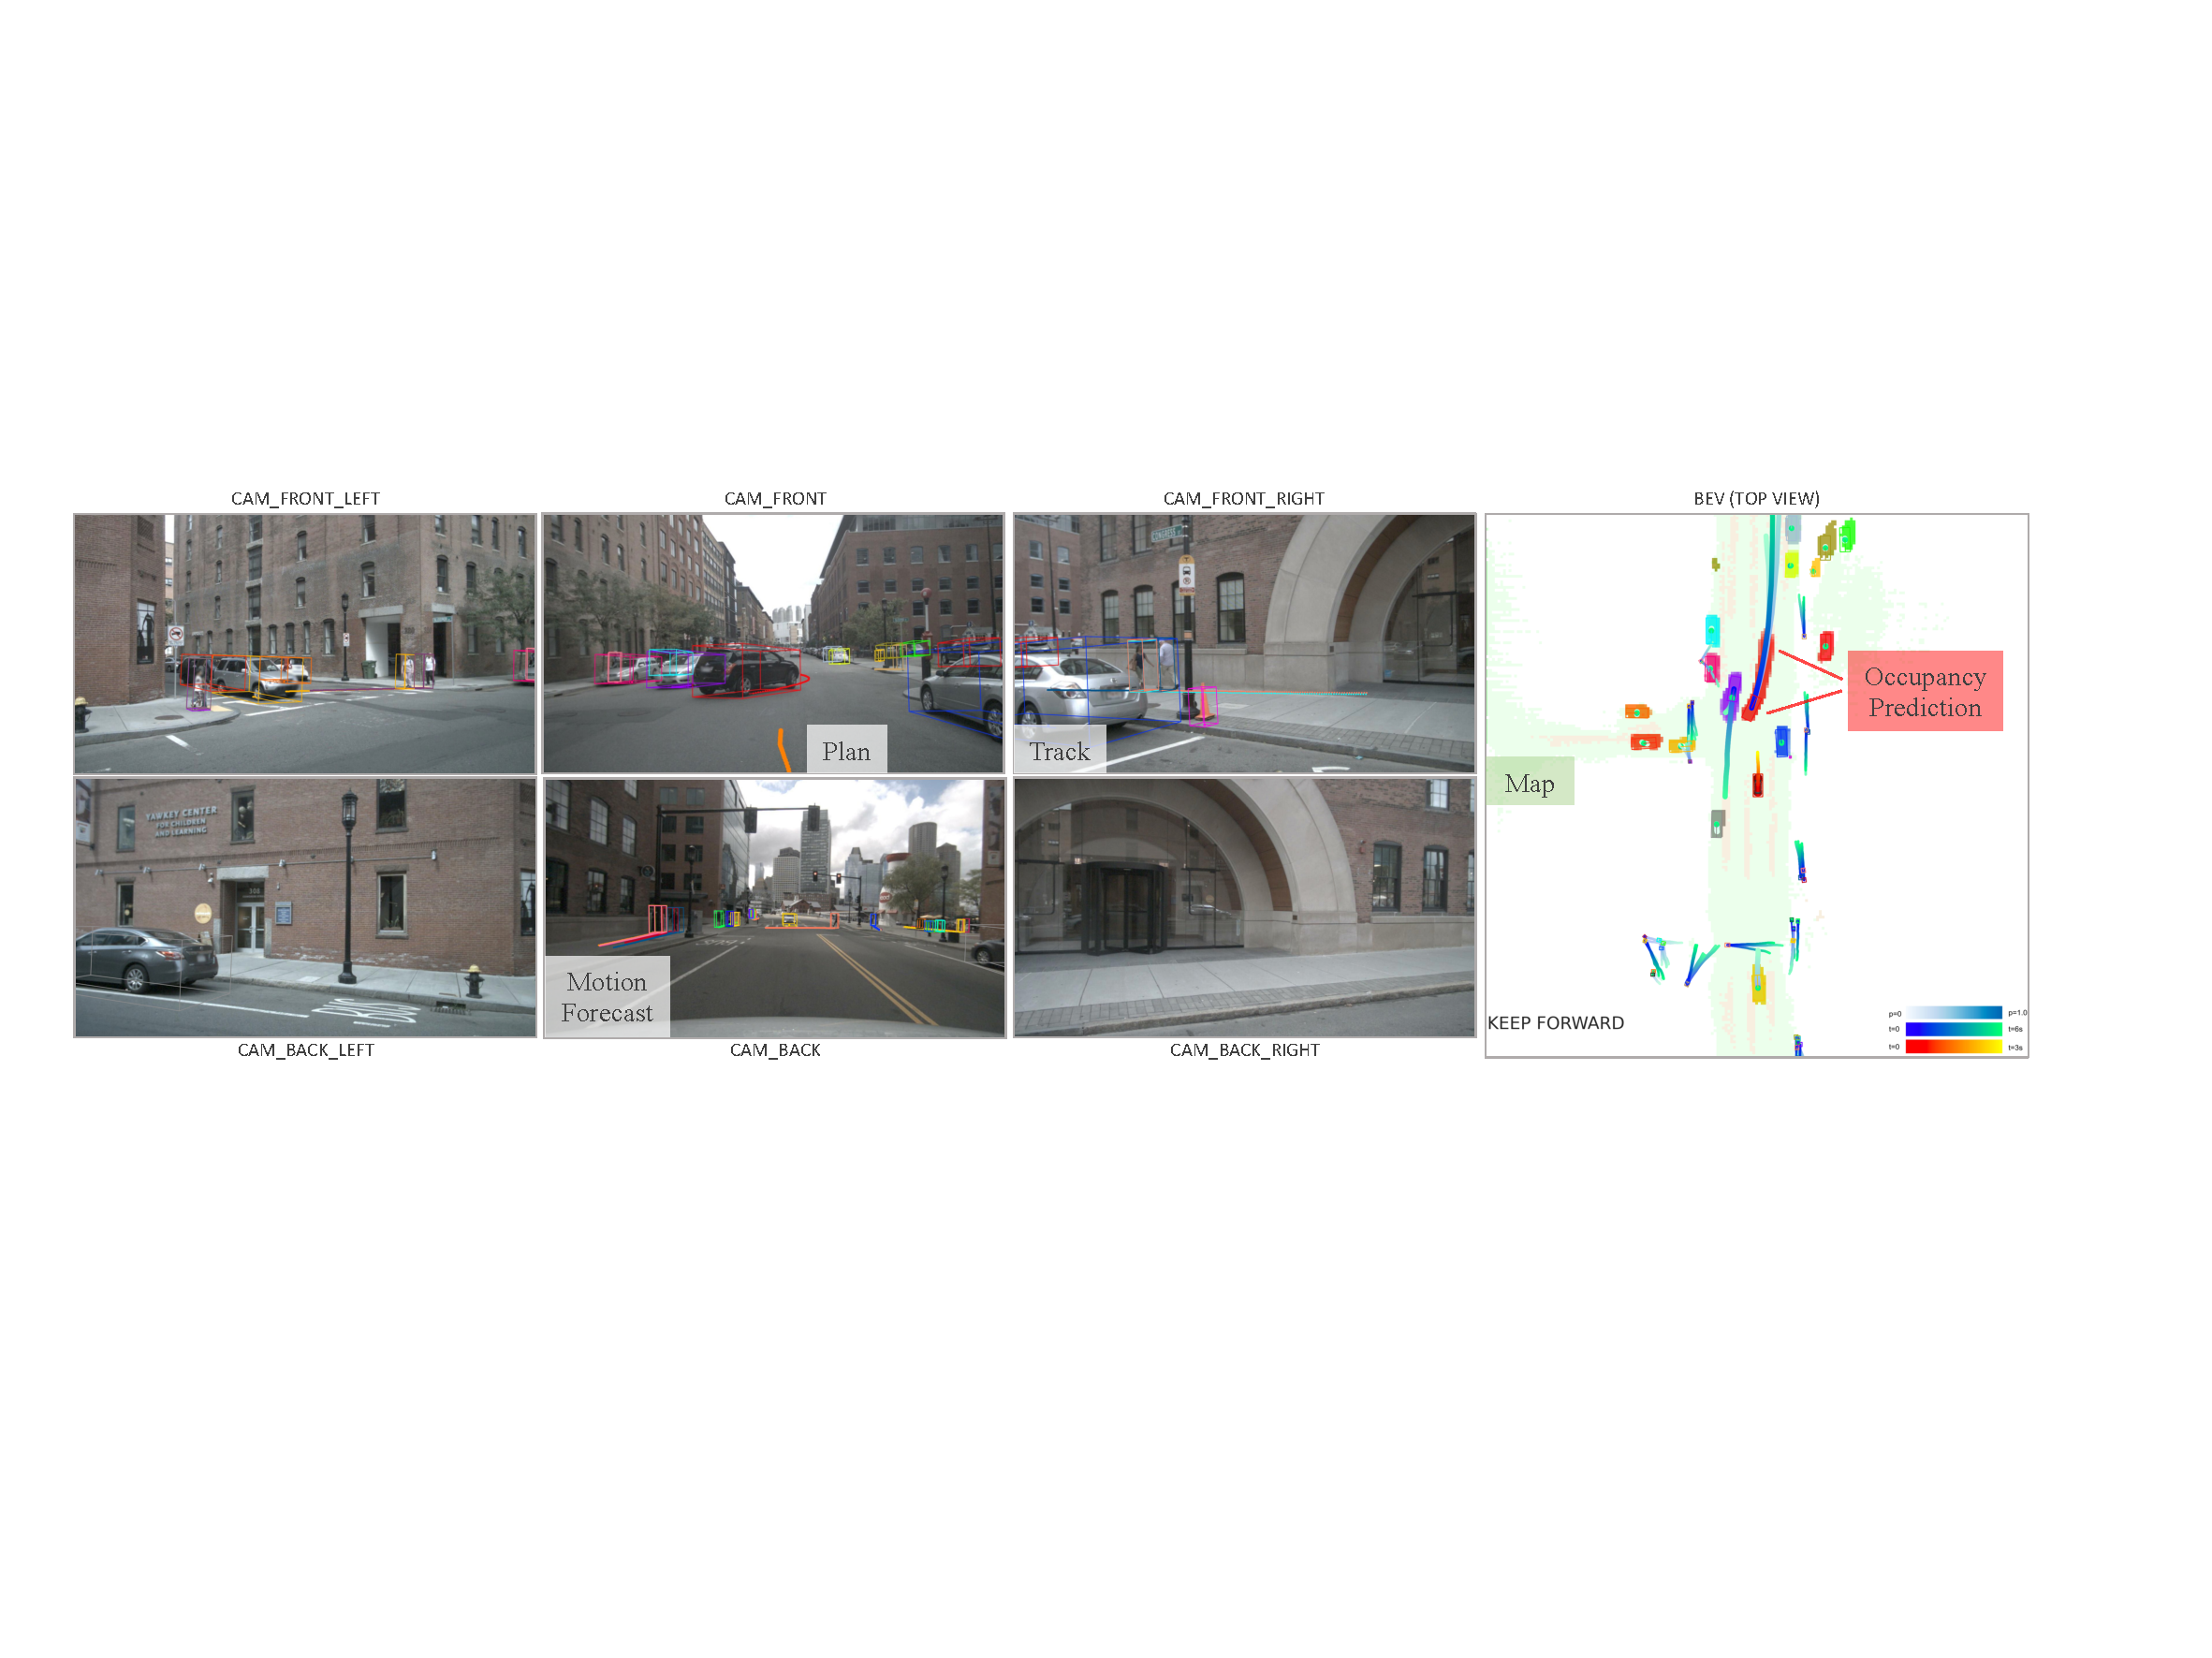
\includegraphics[width=\textwidth]{UniAD/figures/vis3.pdf}
  \vspace{-16pt}
  \caption{\textbf{可视化结果.} 本文展示了所有任务在环视图像和BEV上的结果。运动和占用模块的预测保持一致，在该场景中自车正在避让前方黑色车辆。每个智能体以不同颜色表示。仅选择运动预测中top-1和top-3的轨迹分别用于图像视图和BEV的可视化。
  }
  \label{fig:vis}
\end{figure*}





\subsection{消融实验}
\label{sec:exp-ablation}
\vspace{-4pt}

\paragraph{MotionFormer设计的影响.}
\Cref{tab:abl-traj}显示，\cref{sec:motion-method}中描述的所有设计组件在minADE、minFDE、Miss Rate和minFDE-mAP指标上均对最终性能有所贡献。
%
值得注意的是，旋转的场景级锚点带来了显著的性能提升（minADE降低15.8\%，minFDE降低11.2\%，minFDE-mAP提升1.9个百分点），表明以场景为中心的方式进行运动预测至关重要。
%
智能体-目标点交互通过以规划为导向的视觉特征增强了运动查询，周围智能体也能从考虑自车意图中获益。
%
此外，非线性优化策略通过在端到端场景中考虑感知不确定性，提升了性能（minADE降低5.0\%，minFDE降低8.4\%，MR降低1.0个百分点，minFDE-mAP提升0.7个百分点）。

\vspace{-5pt}
\paragraph{OccFormer设计的影响.}
如\Cref{tab:abl-occ}所示，在没有局部约束的情况下让每个像素关注所有智能体（Exp.2）比无注意力基线（Exp.1）性能略有下降。占用引导的注意力掩码解决了该问题并带来了增益，尤其在近处区域（Exp.3, IoU-n.提升1.0个百分点，VPQ-n.提升1.4个百分点）。
%
此外，使用掩码特征$M^t$而非智能体特征来获取占用特征进一步提升了性能。


\vspace{-5pt}
\paragraph{规划器设计的影响.}
本文在\Cref{tab:abl-planning}中提供了规划器提出设计的消融实验，即关注BEV特征、使用碰撞损失训练和基于占用的优化策略。
%
与先前研究~\cite{hu2021safe,hu2022stp3}类似，安全优先于朴素的轨迹模仿（L2指标），需要更低的碰撞率，该指标在UniAD应用所有设计后得到显著降低。


\section{结论与未来工作}
\label{sec:conclusion}
\vspace{-4pt}

本文讨论了自动驾驶算法框架的系统级设计。
提出了一种以规划为导向的流水线，即UniAD，以追求最终规划目标。本文详细分析了感知和预测中各模块的必要性。为统一各任务，提出了基于查询的设计来连接UniAD中的所有节点，从而为环境中智能体交互提供更丰富的表示。大量实验从各个方面验证了所提出的方法。

\smallskip
\noindent\textbf{局限性与未来工作.} 协调包含多个任务的综合系统并非易事，需要大量计算资源，尤其在使用时序历史训练时。如何设计和精简系统以实现轻量化部署值得未来探索。此外，是否纳入更多任务（如深度估计、行为预测）以及如何将其嵌入系统，也是值得探索的未来方向。

\smallskip
\noindent\textbf{致谢.} 本研究得到了国家重点研发计划（2022ZD0160100）、上海市科学技术委员会（21DZ1100100）和国家自然科学基金（62206172）的部分资助。

%%%%%%%%% REFERENCES
% \clearpage
% \newpage
{\small
\bibliographystyle{ieee_fullname}
\bibliography{egbib}
}

\appendix
\clearpage
\newpage

\noindent\textbf{\large{附录}}

\startcontents
{
    \hypersetup{linkcolor=black}
    \printcontents{}{1}{}
}
\newpage
\section{任务定义}
\label{sec:task-def}

\paragraph{检测与跟踪.}
检测和跟踪是自动驾驶的两个关键感知任务，本文重点在3D空间中表示它们以方便下游使用。3D检测负责在每个时间戳定位周围目标（坐标、长、宽、高等）；跟踪旨在寻找不同时间戳之间不同目标的对应关系并进行时序关联（即为每个智能体分配一致的跟踪ID）。
%
在本文中，某些情况下使用多目标跟踪指代检测和跟踪过程。
%
最终输出是每帧中一系列关联的3D框，其对应特征$Q_A$被传递到运动模块。
%
此外，本文有一个名为\textit{自车查询}的特殊查询用于下游任务，该查询不参与预测-真实匹配过程，而是相应地回归自车位置。

\paragraph{在线建图.} 地图直观地体现了环境的几何和语义信息，在线建图是利用车载传感器数据（本文中为多视角图像）分割有意义的道路元素，以替代离线标注的高精地图。
%
在UniAD中，本文将在线地图建模为四类：车道、可行驶区域、分隔线和人行横道，并在鸟瞰视图（BEV）中进行分割。
%
与$Q_A$类似，地图查询$Q_M$将进一步用于运动预测模块中建模智能体-地图交互。



\paragraph{运动预测.} 预测作为连接感知与规划的桥梁，在整个自动驾驶系统中对确保最终安全性起着重要作用。
%
通常，运动预测是一个独立开发的模块，利用检测到的边界框和高精地图预测智能体的未来轨迹。在大多数当前运动数据集中，边界框来自真实标注~\cite{ettinger2021waymomotion}，这在车载场景中并不现实。
%
而在本文中，运动预测模块将先前编码的稀疏查询（即$Q_{A}$和$Q_{M}$）和密集的BEV特征$B$作为输入，为每个智能体预测未来$T$个时间步中的$\mathcal{K}$条合理轨迹。此外，为兼容端到端和以场景为中心的场景，本文将轨迹预测为相对于每个智能体当前位置的偏移量。
%
在最后的解码MLP之前的智能体特征（已编码历史和未来信息）将被发送到占用模块，用于场景级的未来理解。
%
对于\textit{自车查询}，它同样预测未来的自车运动（实际上提供粗略的规划估计），其特征被规划器用于生成最终目标。

\paragraph{占用预测.} 占用网格图是一种离散化的BEV表示，其中每个单元格包含是否被占用的置信度，占用预测任务旨在发现未来$T_o$个时间步中网格图随多智能体动态的变化。
%
与基于稀疏智能体的运动预测互补，占用预测以整个场景级别的密集方式进行表示。为探究场景如何随稀疏智能体知识演变，本文提出的占用模块同时接收观测到的BEV特征$B$和智能体特征$G^t$作为输入。经过多步智能体-场景交互（详见\cref{sec:imp-detail}），通过占用特征与密集场景特征之间的矩阵乘法生成实例级概率图$\hat{O}_A^t\!\in\!\mathbb{R}^{N_a\!\times\!H\!\times\!W}$。
%
为形成保留智能体身份的全场景占用$\hat{O}^t\!\in\!\mathbb{R}^{H\!\times\!W}$（用于占用评估和下游规划），本文在每个时间步使用逐像素的argmax合并实例级概率，如\cite{carion2020detr}所示。


\paragraph{规划.} 作为最终目标，规划模块综合考虑所有上游结果。
%
传统的工业规划方法通常是基于规则的，由基于各种场景条件（由先前的检测和预测结果描述）的"if-else"状态机构成。
%
在本文基于学习的模型中，以上游\textit{自车查询}和密集BEV特征$B$作为输入，预测总$T_{p}$个时间步的一条轨迹$\hat{\tau}$。然后，利用上游预测的未来占用$\hat{O}$优化轨迹$\hat{\tau}$以避免碰撞并确保最终安全性。

\section{各任务的必要性}
\label{sec:task-necessity}

在感知方面，如PnPNet~\cite{liang2020pnpnet}和ViP3D~\cite{gu2022vip3d}中所做的那样，将\textit{跟踪}纳入循环已被证明可以补充时空特征，为被遮挡的智能体提供历史轨迹，避免下游规划出现灾难性决策。
%
借助高精地图~\cite{zeng2019nmp,sadat2020p3,liang2020pnpnet,gu2022vip3d}和运动预测，规划变得更加准确，向更高层次的智能发展。然而，此类信息构建成本高昂且容易过时，因此产生了在没有高精地图的情况下进行在线\textit{建图}的需求。
%
在预测方面，\textit{运动}预测~\cite{casas2018intentnet, jia2021ide, jia2022temporal, gao2020vectornet, Zhao2020tnt}生成长时序的未来行为，并以稀疏轨迹点输出的形式保留智能体身份。
%
然而，将不可微的框表示集成到后续规划模块中存在挑战~\cite{gu2022vip3d, liang2020pnpnet}。
%
近期一些研究探索了另一种名为\textit{占用}~\cite{thrun1996occgrid}预测的预测任务，以代价图的形式辅助端到端规划。然而，占用中缺乏智能体身份和动态信息，使得建模社交交互以实现安全规划变得不切实际。
%
建模多步密集特征的高计算消耗也导致相比\textit{运动}预测的时间范围短得多。因此，为从两种互补的预测任务中受益以实现安全的\textit{规划}，本文在UniAD中同时融合了以智能体为中心的运动和全场景占用。 


\section{相关工作}
\label{sec:related-work}

\subsection{联合感知与预测}
联合学习感知和预测旨在避免传统模块化独立流程中的级联误差。与单独的运动预测任务类似，它通常有两种输出表示：智能体级边界框和场景级占用网格图。
%
开创性工作FaF~\cite{luo2018faf}预测未来的框并聚合过去信息以生成轨迹段。IntentNet~\cite{casas2018intentnet}将其扩展以推理意图，\cite{djuric2021multixnet, fadadu2022multixnetfusion}进一步以精炼方式预测未来状态。
%
一些方法先进行检测，然后在第二预测阶段利用智能体特征~\cite{casas2020spagnn, li2020contextual, peri2022futuredet}。注意到历史信息被忽略，PnPNet~\cite{liang2020pnpnet}通过估计跟踪关联分数来丰富信息，以避免检测后跟踪范式~\cite{li2022uvtr, shi2022srcn3d, liu2022bevfusion, yang2022qtrack}中采用的不可微优化过程。
%
然而，所有这些方法都依赖检测中的非极大值抑制（NMS），这仍然会导致信息损失。与本文工作密切相关的ViP3D~\cite{gu2022vip3d}采用~\cite{zhang2022mutr3d}中的智能体查询进行预测，并将高精地图作为另一输入。
%
本文在智能体跟踪查询方面遵循了~\cite{zhang2022mutr3d, gu2022vip3d}的理念，同时发展了对目标轨迹的非线性优化，以缓解潜在的不准确感知问题。此外，本文引入了自车查询以更好捕获动态环境中的自车行为，并结合在线建图以避免定位风险或高精地图的高构建成本。

另一种表示即占用网格图，将BEV地图离散化为网格单元，每个单元持有是否被占用的置信度。Wu等人~\cite{wu2020motionnet}估计密集运动场，但无法捕获多模态行为。Fishing Net~\cite{hendy2020fishingnet}也使用多传感器预测确定性的未来BEV语义分割。
%
为解决此问题，P3~\cite{sadat2020p3}提出了未来语义占用的非参数分布，FIERY~\cite{hu2021fiery}设计了首个用于多视角相机的范式。一些方法通过更复杂的建模范式提升了FIERY的性能~\cite{hu2022stp3, akan2022stretchbev, zhang2022beverse}。
%
值得注意的是，这种表示可以轻松扩展到用于碰撞避免的运动规划~\cite{sadat2020p3, casas2021mp3, hu2022stp3}，但丢失了智能体身份特征，且计算负担较重，可能限制预测时间范围。相反，本文利用智能体级信息进行占用预测，并通过统一这两种模式确保准确安全的规划。

\subsection{联合预测与规划} PRECOG~\cite{rhinehart2019precog}提出了一种循环模型，将预测条件建立在自车目标位置上，而PiP~\cite{song2020pip}在考虑完整预设规划轨迹的情况下生成智能体的运动。然而，在现实世界中生成粗略的未来轨迹仍然具有挑战性，\cite{liu2021reactive}为此提出了一种深度结构化模型，从同一组可学习代价中推导出预测和规划。
%
\cite{ivanovic2021mats, huang2022differentiable}将预测模型与经典优化方法相结合。同时，一些运动预测方法通过同时生成未来轨迹隐式包含规划任务~\cite{chai2020multipath, ngiam2021scenetransformer, kamenev2022predictionnet}。
%
类似地，本文在以场景为中心的运动预测模块中编码自车的可能行为，但利用可解释的占用图进一步优化规划以保持安全。


\subsection{端到端运动规划}
自Pomerleau~\cite{pomerleau1988alvinn}使用直接预测控制信号的单一神经网络以来，端到端运动规划一直是一个活跃的研究领域。后续研究取得了重大进展，特别是在使用更深网络~\cite{bojarski2016nvend}、多模态输入~\cite{bansal2018chauffeurnet, codevilla2018cil, prakash2021transfuser}、多任务学习~\cite{wu2022tcp, Chitta2022transfuserpami}、强化学习~\cite{liang2018cirl, kendall2019driveaday, MaRLn, Chekroun2021gri, chen2021wor}和从特定特权知识蒸馏~\cite{chen2020lbc, zhang2021roach, zhang2021lbw}的闭环仿真中。然而，对于这些从传感器数据直接生成控制输出的方法，考虑其鲁棒性和安全保障，从合成环境到实际应用的迁移仍然存在问题~\cite{codevilla2019cilrs, hu2022stp3}。
%
因此研究者旨在显式设计网络的中间表示以促进安全性，其中预测场景如何演变吸引了广泛关注。一些工作~\cite{chitta2021neat, shao2022interfuser, hu2022mile}联合解码规划和BEV语义预测以增强可解释性，而PLOP~\cite{Buhet2020plop}采用多项式公式为自车和邻居提供平滑的规划结果。
%
Cui等人~\cite{cui2021lookout}引入了一种带有多种未来预测集的应急规划器，LAV~\cite{chen2022lav}使用所有车辆的轨迹训练规划器以提供更丰富的训练数据。
%
NMP~\cite{zeng2019nmp}及其变体~\cite{wei2021sanmp}在确定性未来感知之外，估计代价体积以选择成本最小的规划方案。尽管它们可能产生两个模块之间不一致的结果，但代价图设计直观，能够在复杂场景中恢复最终规划。受~\cite{zeng2019nmp}启发，近期工作~\cite{zeng2020dsdnet, sadat2020p3, casas2021mp3, hu2022stp3, hu2021safe}提出了使用学习到的占用预测和手工设计的惩罚项构建代价的模型。
%
然而，它们的性能严重依赖于基于人工经验定制的代价和轨迹采样的分布~\cite{khurana2022ssocc}。
%
与这些方法相反，本文利用自车运动信息而不需要复杂的代价设计，并首次尝试在端到端模型中同时融合跟踪模块和两种预测表示。



\section{符号说明}
\label{sec:notations}
本文在~\Cref{tab:notation}中提供了本文涉及的符号及其形状的查找表以供参考。
\begin{table*}%[hp]
    \definecolor{Gray}{gray}{0.9}
	\begin{center}
			\begin{tabular}{ccl}
				\toprule
				Notation & Shape \& Params. & Description \\
				\midrule
				$Q_o$ & 900 & number of initial object queries \\
				$D$ & 256 & embed dimensions \\
				$B$ & $200 \times 200 \times 256$ &BEV feature encoded by a multi-view framework \\
				$N$ & 6 &number of transformer decoder layers for TrackFormer \\
				$N$ & 6 &number of transformer decoder layers for MapFormer \\
				$N$ & 4 &number of mask decoder layers for MapFormer \\
				$N$ & 3 &number of transformer decoder layers for MotionFormer \\
				$N$ & 5 &number of transformer decoder layers for OccFormer \\
				$N$ & 3 &number of transformer decoder layers for Planner \\
				$N_a$ & \textit{dynamic} &number of agents from TrackFormer \\
				$N_m$ & 300 &number of map queries from MapFormer \\
				$Q_A$ & $N_{a} \times 256$ &agent features from TrackFormer \\
				$P_A$ & $N_{a} \times 256$ &agent positions from TrackFormer \\
				$Q_M$ & $N_{m} \times 256$ &map features from MapFormer \\
				$\mathcal{K}$ & 6 & number of forecasting modality in MotionFormer \\
				% $\mathbf{x_{i,k}}$ & motion forecasting results for agent $i$ under modality $k$ \\
				$\tilde{\mathbf{x}}$ & $T \times 2$ & ground truth for one agent's motion forecasting \\
				$\hat{\mathbf{x}}$ & $N_{a} \times T \times 2$& prediction of motion forecasting \\
				$T$ & 12 &length of prediction timestamps in MotionFormer \\
				$Q_{\text{pos}}$ & $N_{a} \times \mathcal{K} \times 256$ & query position in MotionFormer \\
				$Q_{\text{ctx}}$ & $N_{a} \times \mathcal{K} \times 256$ &query context in MotionFormer \\
				$Q_{a}$ & $N_{a} \times \mathcal{K} \times 256$ &motion query after agent-agent interaction in MotionFormer \\
				$Q_{m}$ & $N_{a} \times \mathcal{K} \times 256$ &motion query after agent-map interaction in MotionFormer \\
				$Q_{g}$ & $N_{a} \times \mathcal{K} \times 256$ &motion query after agent-goal point interaction in MotionFormer \\
				$l$ & - &index of decoder layer \\
				$PE$ & - &sinusoidal position encoding function \\
				$I^s$ & $\mathcal{K} \times T \times 2 $ &scene-level anchor position in MotionFormer \\
				$I^a$ & $\mathcal{K} \times T \times 2 $ &agent-level anchor position in MotionFormer\\
				$\Phi$ & - &kinematic cost function set \\
				$T_o$ & 5 &length of prediction timestamps in OccFormer \\
				$G^t$ & $N_a \times 256$ & agent feature input\\
				$F^t$ &  $200 \times 200 \times 256$ & future state output \\
				$Q_X$ & $N_a \times 256$ & motion query (max-pooled on modality level) from the last layer of MotionFormer \\
				$F_{\text{ds}}^t$ & $25\times 25 \times 256$ & downscaled dense feature\\
				$F_{\text{dec}}^t$ & $200\times 200 \times 256$ &decoded dense feature after convolutional decoder\\
				$D_{\text{ds}}^t$ & $25\times 25 \times 256$ &agent-aware dense feature after pixel-agent interaction\\
				$\hat{O}_A^t$ &$N_{a} \times 200\times 200$ &instance-level probability map\\
				$\hat{O}^t$ &$200\times 200$&classical instance-agnostic occupancy map merged from $\hat{O}_A^t$ for planning\\
				$O_m^t$ & $200\times 200$ &attention mask for pixel-agent interaction\\
				$M^t$ & $N_{a} \times 256$ &mask feature\\
				$U^t$ & $N_{a} \times 256$ &occupancy feature\\
    		$T_p$ & 6 &length of planning timestamps in Planner \\
				$\hat{\tau}$ & $T_p \times 2$ &planned trajectory before the optimization with occupancy prediction \\
				$\tau^*$ & $T_p \times 2 $&ultimate plan output \\
				% $\mathcal{N}$ & - &Gaussian distribution \\
				$\lambda$ & - &hyperparameters in cost functions, target functions, \etc \\
				\bottomrule

			\end{tabular}
	\end{center}
	\vspace{8pt}
	\caption{\textbf{符号与超参数查找表。} 某些符号中的上标$t$表示OccFormer的第$t$个块，在描述中为简洁起见予以省略。}
	\label{tab:notation}
\end{table*} 

\section{实现细节}
\label{sec:imp-detail}

\subsection{检测与跟踪}
\label{sec:detail-track}

本文继承了BEVFormer~\cite{li2022bevformer}的大部分检测设计，该模型使用BEV编码器将图像特征转换为BEV特征$B$，并采用Deformable DETR头~\cite{zhu2020deformabledetr}在$B$上执行检测。为进一步实现端到端跟踪而无需繁重的后关联，本文引入了另一组称为跟踪查询（track queries）的查询，类似于MOTR~\cite{zeng2021motr}，根据分配的跟踪ID持续跟踪先前观测到的实例。以下详细介绍跟踪过程。

\textbf{训练阶段:}
在每个训练序列的起始（即第一帧），所有查询都被视为检测查询并预测所有新出现的物体，这与BEVFormer实质相同。
%
检测查询通过匈牙利算法~\cite{carion2020detr}与真实值进行匹配。它们将通过查询交互模块（QIM）存储和更新，用于下一时间戳作为跟踪查询，遵循MOTR~\cite{zeng2021motr}。
%
在下一时间戳，跟踪查询将根据对应的跟踪ID直接与部分真实目标匹配，而检测查询与剩余的真实目标（新生目标）匹配。为稳定训练，本文采用3D IoU指标筛选匹配的查询。仅与真实框的3D IoU大于一定阈值（实践中为0.5）的预测才会被存储和更新。

\textbf{推理阶段:}
与训练阶段不同，序列的每一帧按顺序送入网络，这意味着跟踪查询的存在时间可能比训练时更长。
%
推理阶段的另一个区别在于查询更新，由于真实值不可用，本文使用分类分数筛选查询（实践中检测查询为0.4，跟踪查询为0.35），而非3D IoU指标。
%
此外，为避免短时遮挡导致的轨迹段中断，本文在推理阶段为轨迹段采用生命周期机制。具体而言，对于每个跟踪查询，只有当其对应分类分数连续一段时间（实践中为2秒）小于0.35时，才被认为完全消失并被移除。


\subsection{在线建图}
\label{sec:detail-map}
遵循~\cite{li2022panopticseg}，本文将地图查询集分解为前景事物查询（thing queries）和背景内容查询（stuff queries）。前景事物查询建模实例级地图元素（即车道、边界和人行横道），并通过二分图匹配与真实值配对，而背景内容查询仅负责语义元素（即可行驶区域），采用类别固定的分配方式。
%
本文将前景事物查询总数设为300，可行驶区域仅设1个背景内容查询。同时，堆叠了6个位置解码器层和4个掩码解码器层（遵循~\cite{li2022panopticseg}中的层结构）。根据经验，本文将位置解码器后的前景事物查询作为地图查询$Q_M$用于下游任务。 


\begin{figure}[t!]
  \centering
  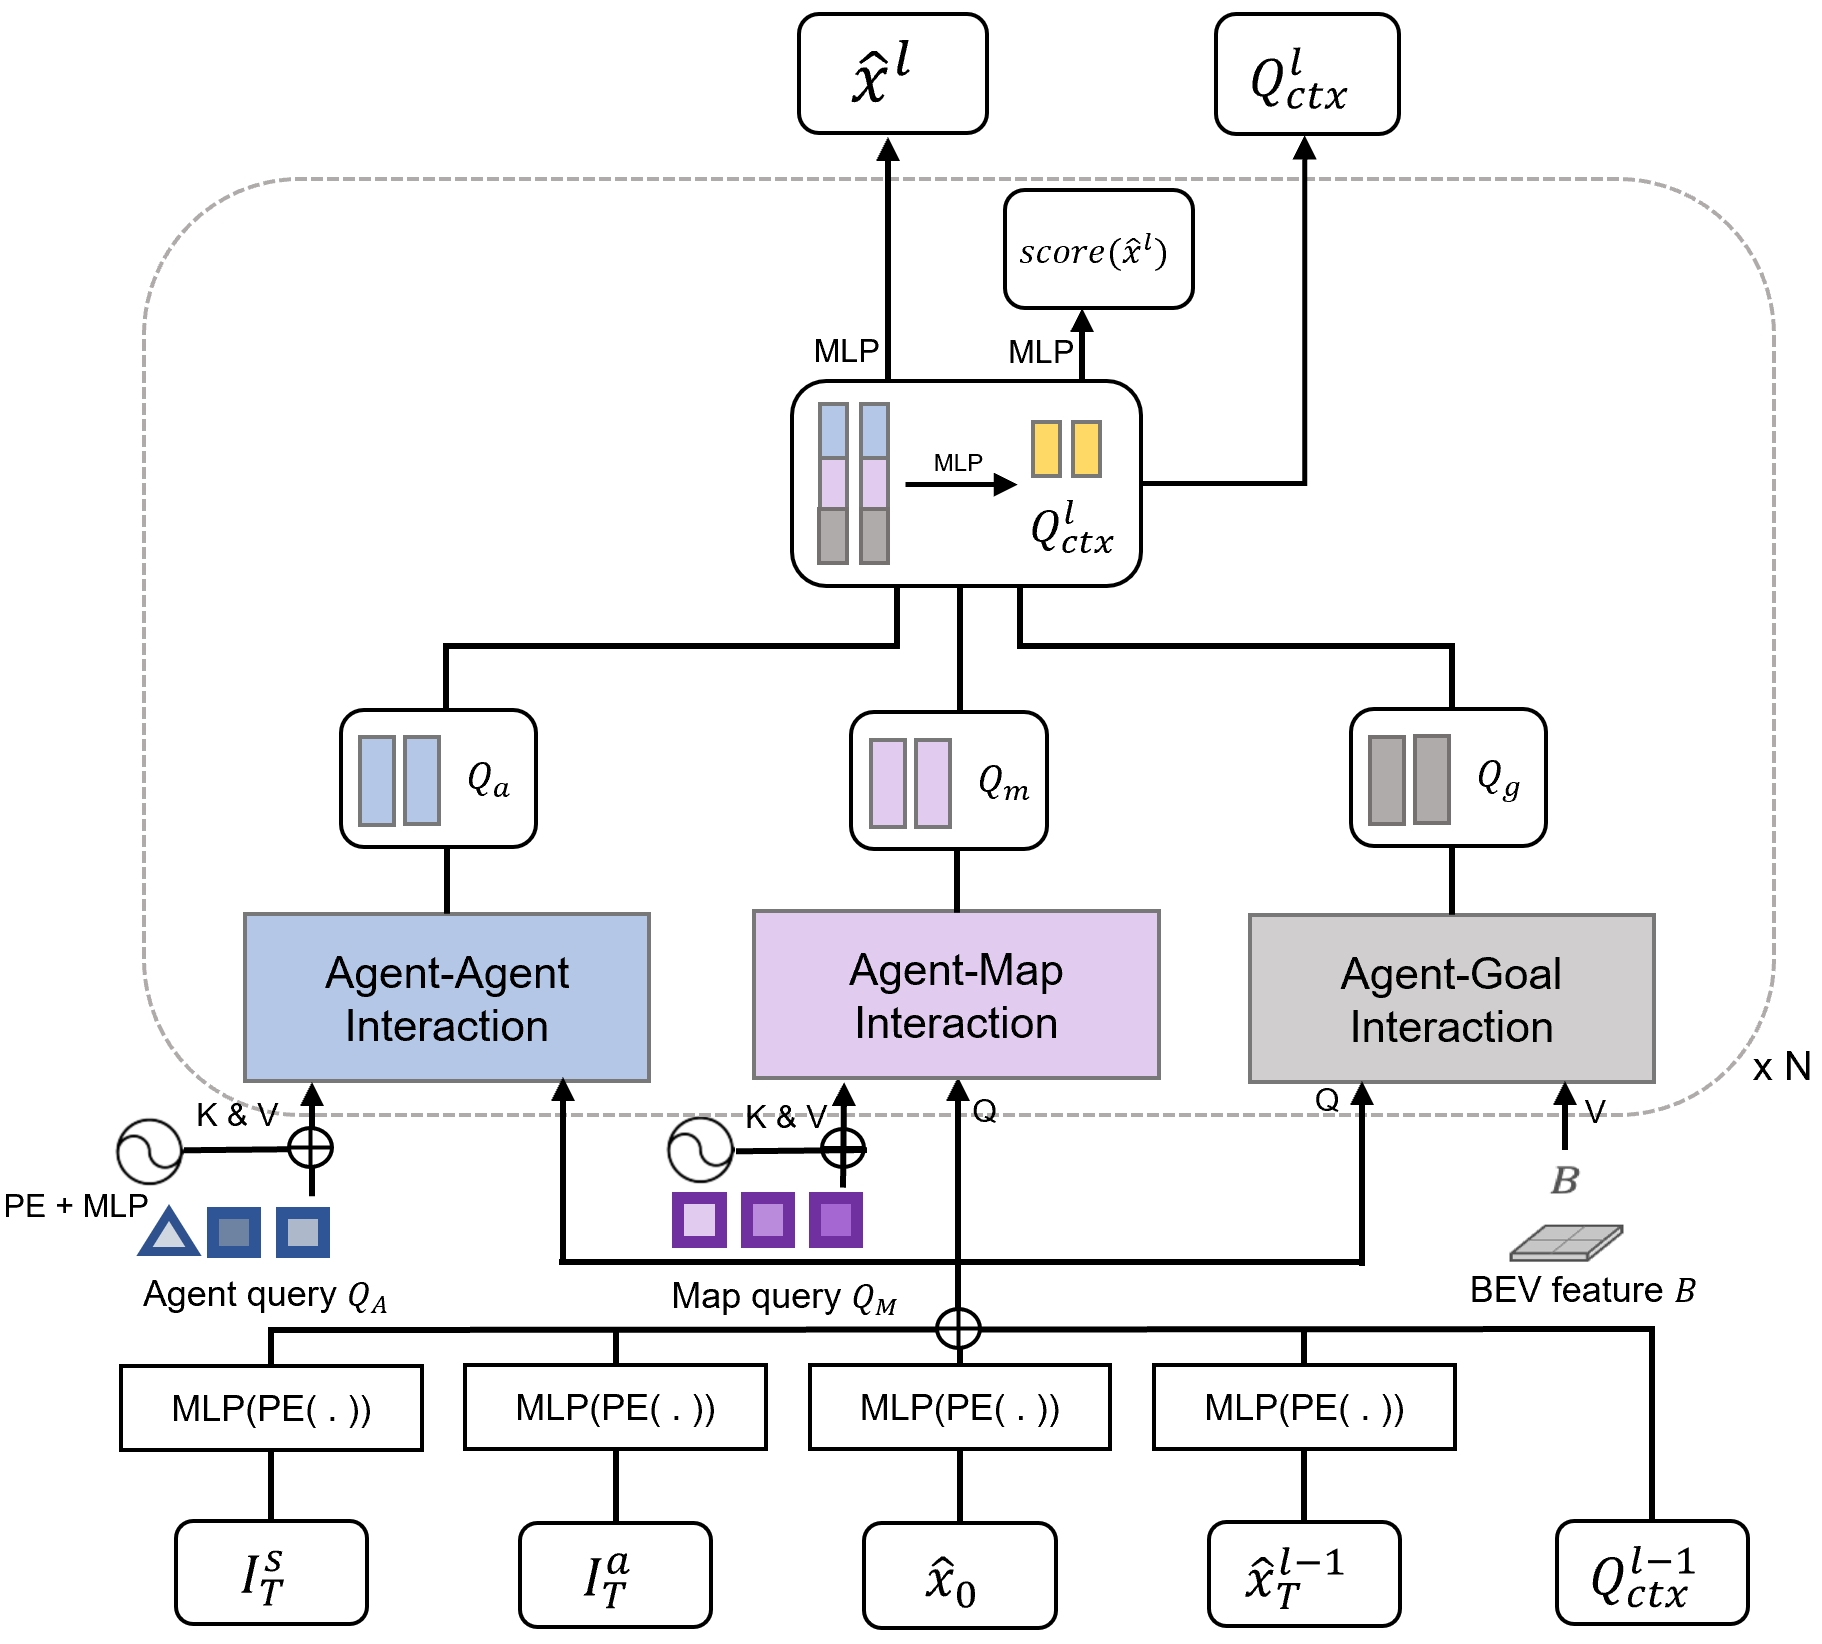
\includegraphics[width=\linewidth]{UniAD/figures/motionformer.jpg}
  \caption{\textbf{MotionFormer.} 它由$N$个堆叠的智能体-智能体、智能体-地图和智能体-目标交互Transformer组成。智能体-智能体和智能体-地图交互模块基于标准Transformer解码器层构建。
  %
  智能体-目标交互模块基于可变形交叉注意力模块~\cite{zhu2020deformabledetr}构建。$I^{s}_{T}$: 场景级锚点终点，$I^{a}_{T}$: 聚类后的智能体级锚点终点，$\hat{x}_0$: 智能体当前位置，$\hat{x}_{T}^{l-1}$: 前一层预测的目标点，$Q_{\text{ctx}}^{l-1}$: 前一层输出的查询上下文。
  }
  \label{fig:motion}
\end{figure}


\begin{figure}[t!]
  \centering
  \scalebox{0.85}{
  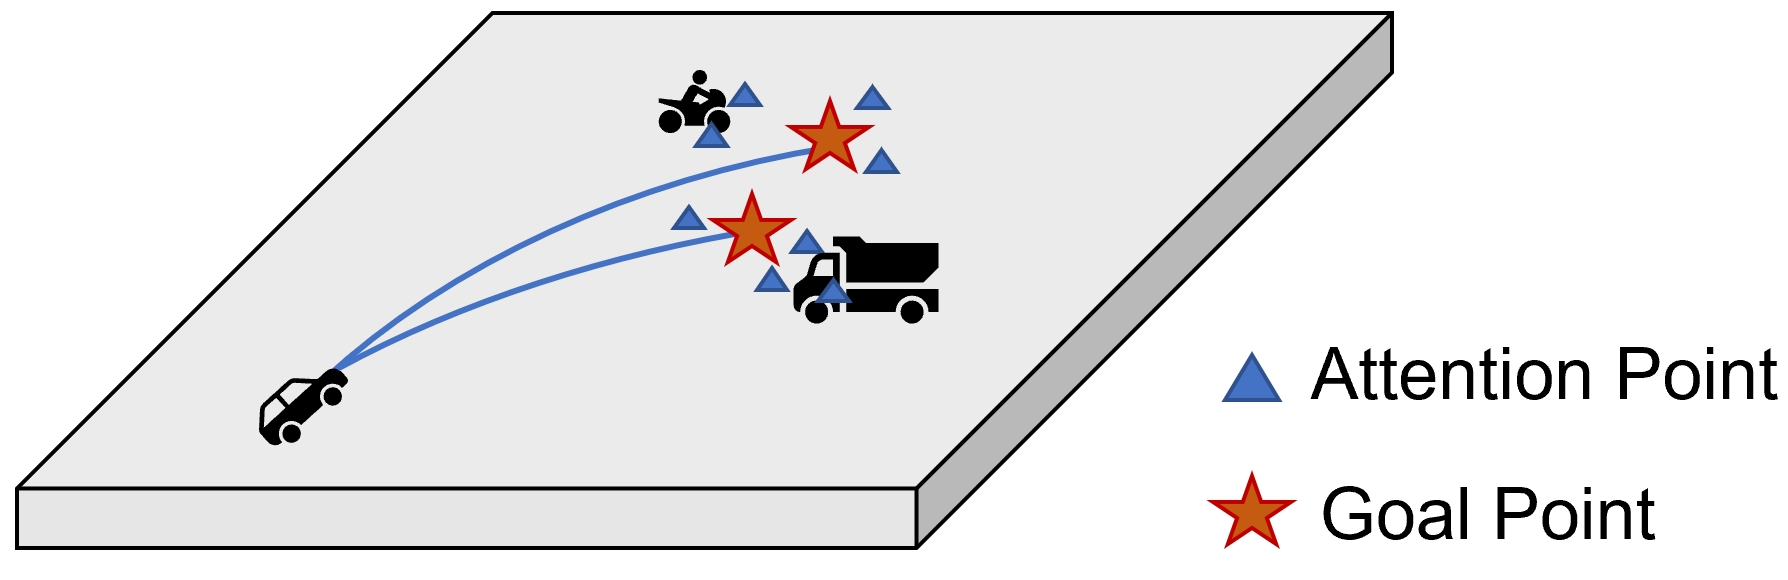
\includegraphics[width=\linewidth]{UniAD/figures/goal-interaction.jpg}
  }
  \caption{\textbf{智能体-目标交互模块示意图.} 通过可变形交叉注意力，在每个智能体目标点附近采样BEV视觉特征。
  }
  \label{fig:goal-interaction}
\end{figure}


\subsection{运动预测}
\label{sec:detail-motion}
为更好说明细节，本文提供了如\cref{fig:motion}所示的示意图。
%
MotionFormer接收$I^{a}_{T}$、$I^{s}_{T}$、$\hat{x}_0$、$\hat{x}_{T}^{l-1} \in \mathbb{R}^{\mathcal{K}\times 2}$来嵌入查询位置，并接收$Q_{ctx}^{l-1}$作为查询上下文。具体而言，锚点通过k-means算法对所有智能体的训练数据进行聚类得到，本文设置$\mathcal{K}\!=\!6$以与输出模态兼容。
%
为嵌入场景级先验，锚点$I^{a}_{T}$根据每个智能体的当前位置和航向角旋转并平移到全局坐标系中，记为$I^{s}_{T}$，如\cref{eq:sl-anchors}所示，
%
\begin{equation}
\label{eq:sl-anchors}
    I_{i, T}^{s} = R_{i} I_{T}^{a} + T_{i},
\end{equation}
%
其中$i$为智能体索引，后文为简洁将其省略。为促进从粗到细的范式，本文还采用了前一层预测的目标点$\hat{x}_{T}^{l-1}$。同时，智能体的当前位置跨模态广播，记为$\hat{x}_0$。
%
然后，对每个先验位置知识应用MLP和正弦位置编码，汇总为查询位置$Q_{\text{pos}} \in \mathbb{R}^{\mathcal{K}\times \mathcal{D}}$，其形状与查询上下文$Q_{ctx}$相同。$Q_{\text{pos}}$和$Q_{\text{ctx}}$共同构成运动查询。本文在整个MotionFormer中将$\mathcal{D}$设为256。
%

如\cref{fig:motion}所示，MotionFormer包含三个主要的Transformer模块，即智能体-智能体、智能体-地图和智能体-目标交互模块。
%
智能体-智能体和智能体-地图交互模块基于标准Transformer解码器层构建，由多头自注意力（MHSA）层和多头交叉注意力（MHCA）层、前馈网络（FFN）以及若干中间残差和归一化层组成~\cite{carion2020detr}。
%
除智能体查询$Q_{A}$和地图查询$Q_M$外，本文还通过正弦位置编码后接MLP层为这些查询添加位置嵌入。
%
智能体-目标交互模块基于可变形交叉注意力模块~\cite{zhu2020deformabledetr}构建，其中先前预测轨迹的目标点（$R_i\hat{x}_{i,T}^{l-1} + T_{i}$）作为参考点，如\cref{fig:goal-interaction}所示。
%
具体而言，本文设置每条轨迹的采样点数为4，每个智能体有6条轨迹，如前所述。
%
每个交互模块的输出特征被拼接并通过MLP层投影到维度$\mathcal{D}\!=\!256$。然后，使用高斯混合模型构建每个智能体的轨迹，其中$\hat{x}_{l} \in \mathcal{R}^{\mathcal{K} \times T \times 5}$。在UniAD中，本文将预测时间范围$T$设为12（6秒）。
%
需要注意的是，仅取最后一个维度的前两个值（即$x$和$y$）作为最终输出轨迹。此外，还预测了每个模态的分数（$score(\hat{x}_{l}) \in \mathcal{R}^{\mathcal{K}}$）。本文将所有模块堆叠$N$次，实践中$N$设为3。




\subsection{占用预测}
\label{sec:detail-occ}

给定上游模块的BEV特征，本文首先通过卷积层将其下采样1/4以实现高效的多步预测，然后传入所提出的OccFormer。OccFormer由$T_o$个顺序块组成，如\cref{fig:occ}所示，其中$T_o\!=\!5$为时间范围（包括当前帧和未来帧），每个块负责生成一个特定帧的占用。
%
与缺乏智能体级知识的先前工作不同，本文提出的方法在展开未来表示时同时融合了密集场景特征和稀疏智能体特征。
%
密集场景特征来自最后一个块的输出（或当前帧的观测特征），并通过卷积层进一步下采样（/8）以减少像素-智能体交互的计算量。
%
稀疏智能体特征来自跟踪查询$Q_A$、智能体位置$P_A$和运动查询$Q_X$的拼接，然后传入时序特定的MLP以获得时序敏感性。
%
本文执行像素级自注意力以建模某些快速变化场景中所需的长期依赖，然后通过将场景的每个像素关注到对应智能体来实现场景-智能体融合。
%
为增强智能体和像素之间的位置对齐，本文使用注意力掩码约束交叉注意力，该掩码由掩码特征与下采样的场景特征进行矩阵乘法生成，其中掩码特征通过MLP编码智能体特征得到。
%
然后将经过注意力处理的密集特征上采样到与输入$F^{t-1}$相同的分辨率（/4），并与$F^{t-1}$相加作为残差连接以保持稳定性。
%
得到的特征$F^{t}$既送入下一个块，也送入卷积解码器以在原始BEV分辨率（/1）下预测占用。重用了掩码特征，并通过另一个MLP形成占用特征，因此实例级占用通过占用特征与解码后的密集特征$F^t_{\text{dec}}$（/1）之间的矩阵乘法生成。
%
需要注意的是，掩码特征的MLP层、占用特征的MLP层和卷积解码器在所有$T_o$个块之间共享，而其他组件在每个块中独立。OccFormer中所有密集特征和智能体特征的维度均为256。


\begin{figure}[t!]
  \centering
  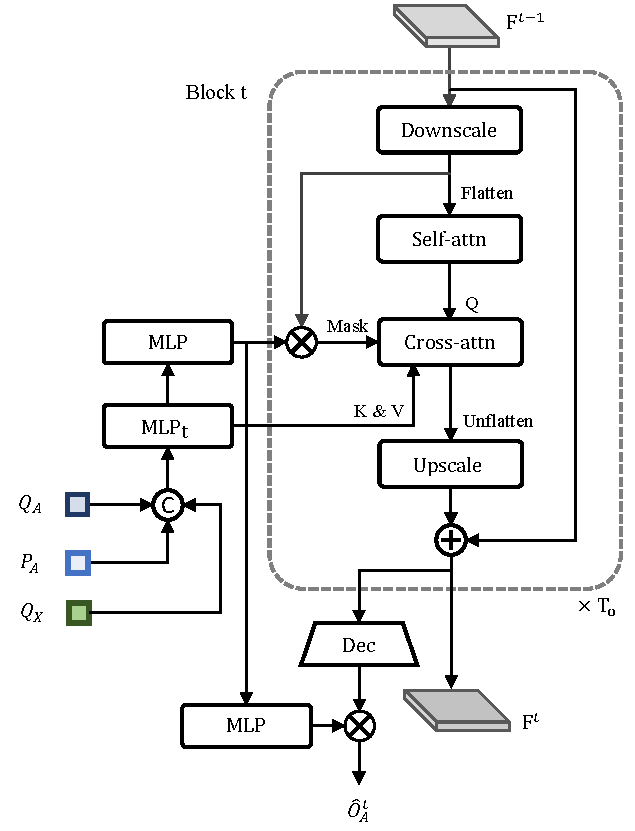
\includegraphics[width=0.9\linewidth]{UniAD/figures/occ_pipeline.pdf}
  \vspace{-8pt}
  \caption{\textbf{OccFormer.} 它由$T_o$个顺序块组成，其中$T_o$为时间范围（包括当前帧和未来帧），每个块负责生成一个特定帧的占用。 
  %
  本文同时融合了密集场景特征和稀疏智能体特征（由上游跟踪查询$Q_A$、智能体位置$P_A$和运动查询$Q_X$编码得到），以将智能体级知识注入未来场景表示。
  %
  在每个块末尾，通过智能体级特征与解码后的密集特征之间的矩阵乘法形成实例级占用$\hat{O}_A^t$。
  %
  }
  \label{fig:occ}
\end{figure}

\subsection{规划}
\label{sec:detail-plan}
如\cref{fig:plan}所示，规划器接收来自跟踪和运动预测模块的自车查询，分别以蓝色三角形和黄色矩形表示。
%
这两个查询与指令嵌入一起，通过MLP层编码，然后经过跨模态维度的最大池化层，选择并聚合最显著的模态特征。
%
BEV特征交互模块基于标准Transformer解码器层构建，堆叠$N$层，此处$N\!=\!3$。具体而言，聚合后的规划查询交叉关注密集BEV特征。
%
更多定性结果见\cref{sec:exp-qualitative}，展示了该模块的有效性。为嵌入位置信息，本文将规划查询与学习的位置嵌入融合，并将BEV特征与正弦位置编码融合。
%
然后通过MLP层回归规划轨迹，记为$\hat{\tau} \in \mathcal{R}^{T_{p} \times 2}$。此处$T_{p}\!=
\!6$（3秒）。最后，设计了用于避障的碰撞优化器，接收预测的占用$\hat{O}$和轨迹$\hat{\tau}$作为输入，如正文\cref{eq:col-cost}所示。设置$d\!=\!5$，$\sigma\!=\!1.0$，$\lambda_{\text{coord}}\!=\!1.0$，$\lambda_{\text{obs}}\!=\!5.0$。

\begin{figure}[t!]
  \centering
  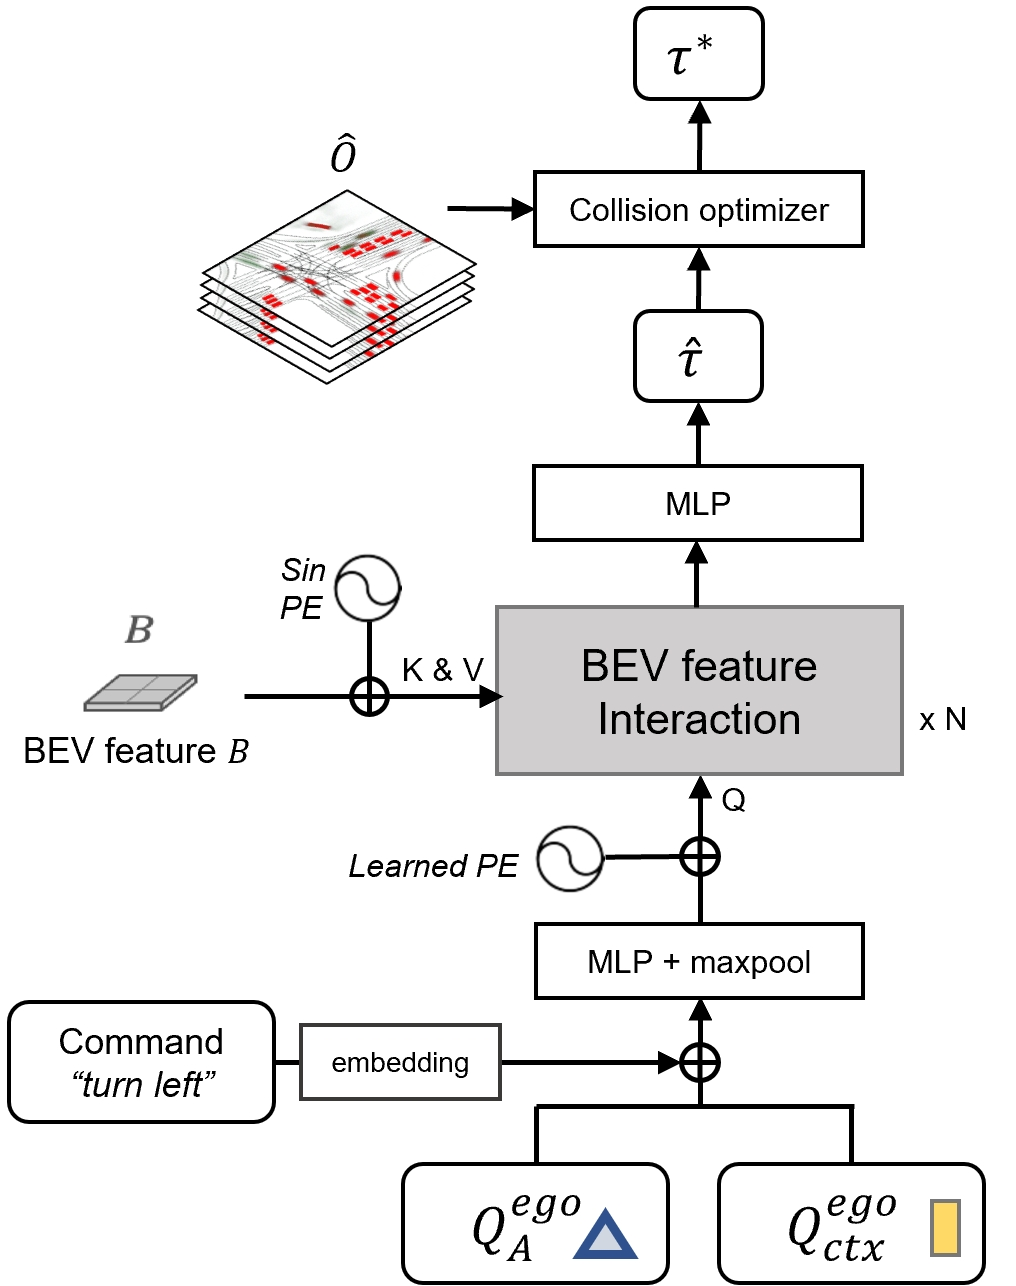
\includegraphics[width=0.8\linewidth]{UniAD/figures/planner.jpg}
  \caption{\textbf{规划器.}
  $Q_A^{\text{ego}}$和$Q_{\text{ctx}}^{\text{ego}}$分别来自跟踪和运动预测模块的\textit{自车查询}。
  %
  它们与高级指令一起通过MLP层编码，然后经过跨模态维度的最大池化层，选择并聚合最显著的模态特征。
  %
  BEV特征交互模块基于标准Transformer解码器层构建，堆叠$N$层。 
  }
  \label{fig:plan}
\end{figure}



\subsection{训练细节}
\label{sec:detail-train}

\paragraph{联合学习.}
UniAD采用两阶段训练，实验发现这种方式更加稳定。
在\textbf{第一阶段}，预训练包括跟踪和在线建图在内的感知任务，以稳定感知预测。
%
具体而言，加载预训练的BEVFormer~\cite{li2022bevformer}权重到UniAD以加速收敛，包括图像骨干网络、FPN、BEV编码器和检测解码器，但不包括目标查询嵌入（由于额外的\textit{自车查询}）。停止图像骨干网络中的梯度反向传播以减少内存成本，并使用跟踪和在线建图损失训练UniAD共6个周期，如下所示：
%
\begin{equation}
\label{eq:all-loss-1}
    L_1 = L_{\text{track}} + L_{\text{map}}.
\end{equation}
%
在\textbf{第二阶段}，同样保持图像骨干网络冻结，并额外冻结用于视图变换（图像视图到BEV）的BEV编码器，以在更多下游模块的情况下进一步减少内存消耗。此时UniAD使用所有任务损失（包括跟踪、建图、运动预测、占用预测和规划）训练20个周期（为效率起见，在正文的各种消融研究中训练8个周期）：
%
\begin{equation}
\label{eq:all-loss}
    L_2 = L_{\text{track}} + L_{\text{map}} + L_{\text{motion}} + L_{\text{occ}} + L_{\text{plan}}.
\end{equation}
%
$L_1$和$L_2$各项中的详细损失函数和超参数将在下文分别描述。在两个阶段中，每个训练序列（每步）用于跟踪和BEV特征聚合\cite{li2022bevformer}的长度为5（为效率起见，消融研究中为3）。


\paragraph{检测与跟踪损失.} 遵循BEVFormer~\cite{li2022bevformer}，每个配对结果采用\textit{Hungarian损失}，它是用于类别标签的Focal损失~\cite{lin2017focal}和用于3D框定位的$l_1$损失的线性组合。
%
在匹配策略方面，新生查询的候选框通过二分图匹配与真实目标配对，而跟踪查询的预测继承先前帧分配的真实索引。
%
具体而言，$L_{\text{track}} = \lambda_{\text{focal}} L_{\text{focal}} + \lambda_{l_1} L_{l_1}$，其中$\lambda_{\text{focal}}\!=\!2$，$\lambda_{l_1}\!=\!0.25$。

\paragraph{在线建图损失.} 如~\cite{li2022panopticseg}所述，这包括针对车道、分隔线和边界的前景事物损失，以及针对可行驶区域的背景内容损失，其中Focal损失负责分类，L1损失负责前景事物边界框，Dice损失和GIoU损失\cite{rezatofighi2019giou}负责分割。
%
具体而言，$L_{\text{map}} = \lambda_{\text{focal}} L_{\text{focal}} + \lambda_{l_1} L_{l_1} + \lambda_{\text{giou}} L_{\text{giou}} + \lambda_{\text{dice}} L_{\text{dice}}$，其中$\lambda_{\text{focal}}\!=\!\lambda_{\text{giou}}\!=\!\lambda_{\text{dice}}\!=\!2$，$\lambda_{l_1}\!=\!0.25$。

\paragraph{运动预测损失.} 与大多数先前方法类似，本文将多模态轨迹建模为高斯混合分布，并使用多路径损失（multi-path loss）~\cite{chai2020multipath, varadarajan2021multipath++}，包括分类分数损失$L_{\text{cls}}$和负对数似然损失项$L_{\text{nll}}$，$\lambda$表示对应权重：
%
$L_{\text{motion}} = \lambda_{\text{cls}} L_{\text{cls}} + \lambda_{\text{reg}} L_{\text{nll}}$，其中$\lambda_{\text{cls}}\!\!=\!\!\lambda_{\text{reg}}\!\!=\!\!0.5$。
%
为确保轨迹的时间平滑性，本文首先预测每个时间步的智能体速度，然后随时间累积以获得最终轨迹~\cite{jia2022temporal}。

\paragraph{占用预测损失.} 实例级占用预测的输出是每个智能体的二值分割，因此采用二值交叉熵和Dice损失~\cite{milletari2016dice}作为占用损失。
%
形式上，$L_{\text{occ}} = \lambda_{\text{bce}} L_{\text{bce}} + \lambda_{\text{dice}} L_{\text{dice}}$，其中$\lambda_{\text{bce}}\!=\!5$，$\lambda_{\text{dice}}\!=\!1$。
%
此外，由于像素-智能体交互模块中的注意力掩码可视为粗略预测，本文采用相同形式的辅助占用损失进行监督。


\paragraph{规划损失.} 安全性是规划中最关键的因素。因此，除了朴素的模仿$l_2$损失外，本文还采用另一种碰撞损失，使规划轨迹远离障碍物，如下所示：
\begin{equation}
\label{eq:col-iouloss}
    L_{\text{col}}(\hat{\tau}, \delta) = \sum_{i, t} \texttt{IoU}(box(\hat{\tau}_{t}, w+\delta, l+\delta), b_{i, t})),
\end{equation}
%
\begin{equation}
\label{eq:plan-loss}
    L_{\text{plan}} = \lambda_{\text{imi}} |\hat{\tau}, \tilde{\tau}|_2 + \lambda_{\text{col}} \sum_{(\omega,\delta) } \omega  L_{\text{col}}(\hat{\tau}, \delta),
\end{equation}
其中$\lambda_{\text{imi}}\!=\!1$，$\lambda_{\text{col}}\!=\!2.5$，$(\omega,\delta)$是考虑额外安全距离的权重-数值对，$box(\hat{\tau}_{t}, w\!+\!\delta, l\!+\!\delta)$
表示在时间戳$t$增大尺寸的自车边界框，以保持更大的安全距离，$b_{i,t}$表示场景中预测的每个智能体。实践中，设置$(\omega,\delta)$为$(1.0, 0.0), (0.4, 0.5), (0.1, 1.0)$。


\section{实验设置}
\label{sec:exp}

\subsection{实验协议}
\label{sec:exp-protocol}

本文在两个阶段均遵循BEVFormer~\cite{li2022bevformer}的大多数基本训练设置，批次大小为1，学习率为$2\!\times\!10^{-4}$，骨干网络的学习率倍率为0.1，使用AdamW优化器~\cite{adamw}，权重衰减为$1\!\times\!10^{-2}$。
%
默认BEV尺寸为$200\!\times\!200$，覆盖X轴和Y轴[-51.2$m$, 51.2$m$]的BEV范围，间隔为0.512$m$。
%
更多与特征维度相关的超参数见\Cref{tab:notation}。实验使用16张NVIDIA Tesla A100 GPU进行。


\subsection{评估指标}
\label{sec:exp-metric}
\paragraph{多目标跟踪.}
遵循标准评估协议，本文使用\textbf{AMOTA}（平均多目标跟踪准确率）、\textbf{AMOTP}（平均多目标跟踪精度）、\textbf{Recall}（召回率）和\textbf{IDS}（身份切换次数）来评估UniAD在nuScenes数据集上的3D跟踪性能。
%
AMOTA和AMOTP通过集成所有召回率上的MOTA（多目标跟踪准确率）和MOTP（多目标跟踪精度）值计算：
%
\begin{equation}
    \label{eq:amota}
    \text{AMOTA} = \frac{1}{n-1}\sum_{r\in\{\frac{1}{n-1}, \frac{2}{n-1},...,1\}}
    \text{MOTA}_{r},
\end{equation}
%
\begin{equation}
    \label{eq:mota}
    \text{MOTA}_{r} = \mathop{\max}(0, 1-\frac{\text{FP}_{r}+\text{FN}_{r}+\text{IDS}_{r}-(1-r)\text{GT}}{r\text{GT}}),
\end{equation}
%
其中$\text{FP}_{r}$、$\text{FN}_{r}$和$\text{IDS}_{r}$分别表示在对应召回率$r$下计算的假阳性、假阴性和身份切换次数。GT表示该帧中真实目标的数量。AMOTP定义如下：
%
\begin{equation}
    \label{eq:amotp}
    \text{AMOTP} =
    \frac{1}{n-1}\sum_{r\in\{\frac{1}{n-1}, \frac{2}{n-1},...,1\}}
    \frac{\sum_{i,t}d_{i,t}}{\text{TP}_r},
\end{equation}
%
其中$d_{i,t}$表示匹配轨迹$i$在时间戳$t$的位置误差（在$x$和$y$轴上），$\text{TP}_r$为对应召回率$r$下的真阳性数量。

\paragraph{在线建图.} 本文在线建图任务有四个类别：车道、边界、人行横道和可行驶区域。计算每类网络输出与真实地图之间的交并比（\textbf{IoU}）指标。

\paragraph{运动预测.} 一方面，遵循标准运动预测协议，本文采用传统指标，包括\textbf{minADE}（最小平均位移误差）、\textbf{minFDE}（最小最终位移误差）和\textbf{MR}（缺失率）。与先前工作~\cite{luo2018faf, liang2020pnpnet, peri2022futuredet}类似，这些指标仅在匹配的TP内计算，所有实验中匹配阈值设为1.0$m$。
%
对于MR，缺失FDE阈值设为2.0$m$。另一方面，本文还采用了近期提出的端到端指标，即\textbf{EPA}（端到端预测准确率）~\cite{gu2022vip3d}和\textbf{minFDE-AP}~\cite{peri2022futuredet}。
%
对于EPA，使用与ViP3D~\cite{gu2022vip3d}相同的设置以确保公平比较。对于minFDE-AP，为简单起见，不将真实值分为多个区间（静态、线性和非线性运动子类别）。
%
具体而言，仅当目标的感知位置及其min-FDE均在距离阈值内（分别为1.0$m$和2.0$m$）时，才将其计为AP（平均精度）计算的TP。
%
与先前工作类似，本文将汽车、卡车、工程车辆、公交车、拖车、摩托车和自行车合并为车辆类别，实验中提供的所有运动预测指标均在车辆类别上评估。

\begin{table*}[t!]
    \definecolor{Gray}{gray}{0.9}
	\begin{center}
		\resizebox{\textwidth}{!}{
			\begin{tabular}{l|c|ccc|cc|cccc|cccc|cc}
				\toprule
				\multirow{2}{*}{Methods} & 
				\multirow{2}{*}{Encoder} & 
				\multicolumn{3}{c|}{Tracking} & 
				\multicolumn{2}{c|}{Mapping} & 
				\multicolumn{4}{c|}{Motion Forecasting} & 
				\multicolumn{4}{c|}{Occupancy Prediction} & \multicolumn{2}{c}{Planning} \\
				& & AMOTA$\uparrow$ & AMOTP$\downarrow$ &IDS$\downarrow$ & IoU-lane$\uparrow$ & IoU-road$\uparrow$ & minADE$\downarrow$ & minFDE$\downarrow$ & MR$\downarrow$ & EPA$\uparrow$ & IoU-n.$\uparrow$ & IoU-f.$\uparrow$ & VPQ-n.$\uparrow$ & VPQ-f.$\uparrow$ & avg.L2$\downarrow$ & avg.Col.$\downarrow$ \\
				\midrule
				\textbf{\algname}-S & R50  & 0.241 & 1.488 & 958 & 0.315 & 0.689 & 0.788 & 1.126 & 0.156 & 0.381 & 59.4 & 35.6 & 49.2 & 28.9 & 1.04 & 0.32 \\
				\textbf{\algname}-B & R101 & 0.359 & 1.320 & \textbf{906} & 0.313 & 0.691 & \textbf{0.708} & \textbf{1.025} & \textbf{0.151} & 0.456 & 63.4 & 40.2 & 54.7 & 33.5 & 1.03 & 0.31 \\
				\textbf{\algname}-L & V2-99$^\ast$  & \textbf{0.409} & \textbf{1.259} & 1583 & \textbf{0.323} & \textbf{0.709} & 0.723 & 1.067 & 0.158 & \textbf{0.508} & \textbf{64.1} & \textbf{42.6} & \textbf{55.8} & \textbf{36.9} & \textbf{1.03} & \textbf{0.29}\\
				\bottomrule
			\end{tabular}
		}
	\end{center}
	\vspace{-10pt}
	\caption{\textbf{三种UniAD变体的比较.}
	$\ast$: 使用额外深度数据进行预训练~\cite{park2021dd3d}。
        }
	\label{tab:SOTA_2}
\end{table*} 

\paragraph{占用预测.} 本文按照~\cite{hu2021fiery, zhang2022beverse}在场景级和实例级评估预测占用质量。具体而言，\textbf{IoU}衡量与实例无关的全场景类别分割，而视频全景质量（\textbf{VPQ}）~\cite{kim2020vpq}考虑每个实例的存在性和时间一致性。VPQ指标计算如下：
\begin{equation}
    \text{VPQ} = \sum_{t=0}^H \frac{\sum_{(p_t,q_t) \in \text{TP}_t} \texttt{IoU}(p_t,q_t)}{|\text{TP}_t| + \frac{1}{2}|\text{FP}_t| + \frac{1}{2}|\text{FN}_t|},
\end{equation}
其中$H$为未来时间范围，如~\cite{hu2021fiery, zhang2022beverse}中设置$H\!=\!4$（因此$T_o\!=\!5$，包含当前时间戳），覆盖2Hz下2.0$s$的连续数据。$\text{TP}_t$、$\text{FP}_t$和$\text{FN}_t$分别为时间戳$t$的真阳性、假阳性和假阴性集合。两个指标均在两种不同的BEV范围内评估，\textbf{near}（近处，"n."）为自车周围$30m\!\times\!30m$，\textbf{far}（远处，"f."）为$100m\!\times\!100m$。本文对当前步（$t\!=\!0$）和未来4步的结果在两个指标上一起评估。




\begin{table}[t!]
    \definecolor{Gray}{gray}{0.9}
	\begin{center}
        \scalebox{0.65}{
			\begin{tabular}{l|cccccc|ccc}
				\toprule
				ID & Det. & Track & Map & Motion & Occ. & Plan &
				\#Params & FLOPs & FPS  \\
				\midrule
				0\cite{zhang2022beverse} & \cmark &  & \cmark &  & \cmark &  & 102.5M  & 1921G & - \\
				\midrule
				1 & \cmark &  &  &  &  &  &  65.9M & 1324G & 4.2  \\
				2 & \cmark & \cmark &  &  &  &  & 68.2M & 1326G & 2.7  \\
				3 & \cmark & \cmark & \cmark &  &  &  & 95.8M & 1520G & 2.2  \\
				4 & \cmark & \cmark & \cmark & \cmark &  &  & 108.6M & 1535G & 2.1  \\
				5 & \cmark & \cmark & \cmark & \cmark & \cmark &  & 122.5M & 1701G & 2.0  \\
				6 & \cmark & \cmark & \cmark & \cmark & \cmark & \cmark & 125.0M & 1709G &  1.8 \\
				\bottomrule
			\end{tabular}
		}
	\end{center}
	\vspace{-10pt}
	\caption{\textbf{不同模块的计算复杂度和运行时间.} ID.1类似于原始BEVFormer~\cite{li2022bevformer}，ID.0（BEVerse-Tiny）~\cite{zhang2022beverse}是一个MTL框架。}
	\label{tab:abl-module-computation}
\end{table} 

\paragraph{规划.} 采用与ST-P3~\cite{hu2022stp3}相同的指标，即不同时间戳的\textbf{L2误差}和\textbf{碰撞率}。


\subsection{模型复杂度与计算成本}
本文在Nvidia Tesla A100 GPU上测量了UniAD的复杂度和运行时间，如\Cref{tab:abl-module-computation}所示。
%
与原始BEVFormer检测器（ID.1）相比，尽管任务的解码器部分带来了一定参数量的增加，但计算复杂度主要来自编码器部分。
%
本文还与最近的BEVerse~\cite{zhang2022beverse}进行了比较。UniAD拥有更多任务，实现了更优性能，且FLOPs\textit{更低}，说明额外计算成本的预算可承受。




\subsection{模型规模}
\label{sec:exp-sota2}
本文提供了UniAD在三种不同模型规模下的变体，如\Cref{tab:SOTA_2}所示。选择的图像视图特征提取骨干网络分别为ResNet-50\cite{he2016resnet}、ResNet-101和VoVNet 2-99\cite{lee2019vovnet}，对应\algname-S、\algname-B和\algname-L。
%
由于模型规模（图像编码器）主要影响BEV特征质量，可以观察到感知分数随骨干网络增大而提升，进而带来更好的预测和规划性能。

\subsection{定性结果}
\label{sec:exp-qualitative}

\paragraph{注意力掩码可视化.} 为探究内部机制并展示可解释性，本文可视化了规划器中交叉注意力模块的注意力掩码。如\cref{fig:vis-supp-attn_mask}所示，预测的跟踪边界框、规划轨迹和真实高精地图（HD Map）被渲染作为参考，注意力掩码叠加在其上方。
%
从左到右，展示了同一时间序列中两个连续帧但具有不同导航指令的情况。可以观察到规划轨迹根据指令变化很大。同时，大量注意力集中在目标车道以及为自车让行的关键智能体上。

\paragraph{不同场景可视化.}
本文提供了更多场景的可视化结果，包括城市区域巡航（\cref{fig:vis-supp-best}）、关键案例（\cref{fig:vis-supp-critical}）和避障场景（\cref{fig:vis-planning-obs-avoid}）。
%
以规划为导向的设计的一个有力证据如\cref{fig:vis-supp-failure1}所示，前置模块中出现不准确结果，而后续任务仍然可以恢复。
%
类似地，本文展示了所有任务在环视图像、BEV以及规划器注意力掩码上的结果。
%
同时提供演示视频\footnote{\url{https://opendrivelab.github.io/UniAD/}}供参考。

\paragraph{失败案例} 对自动驾驶算法理解其弱点并指导未来工作至关重要，本文在此展示UniAD的一些失败案例。
%
UniAD的失败案例主要出现在所有模块都受到影响的长尾场景中，如\cref{fig:vis-supp-failure2}和\cref{fig:vis-supp-failure3}所示。


\begin{figure*}[t!]
  \centering
  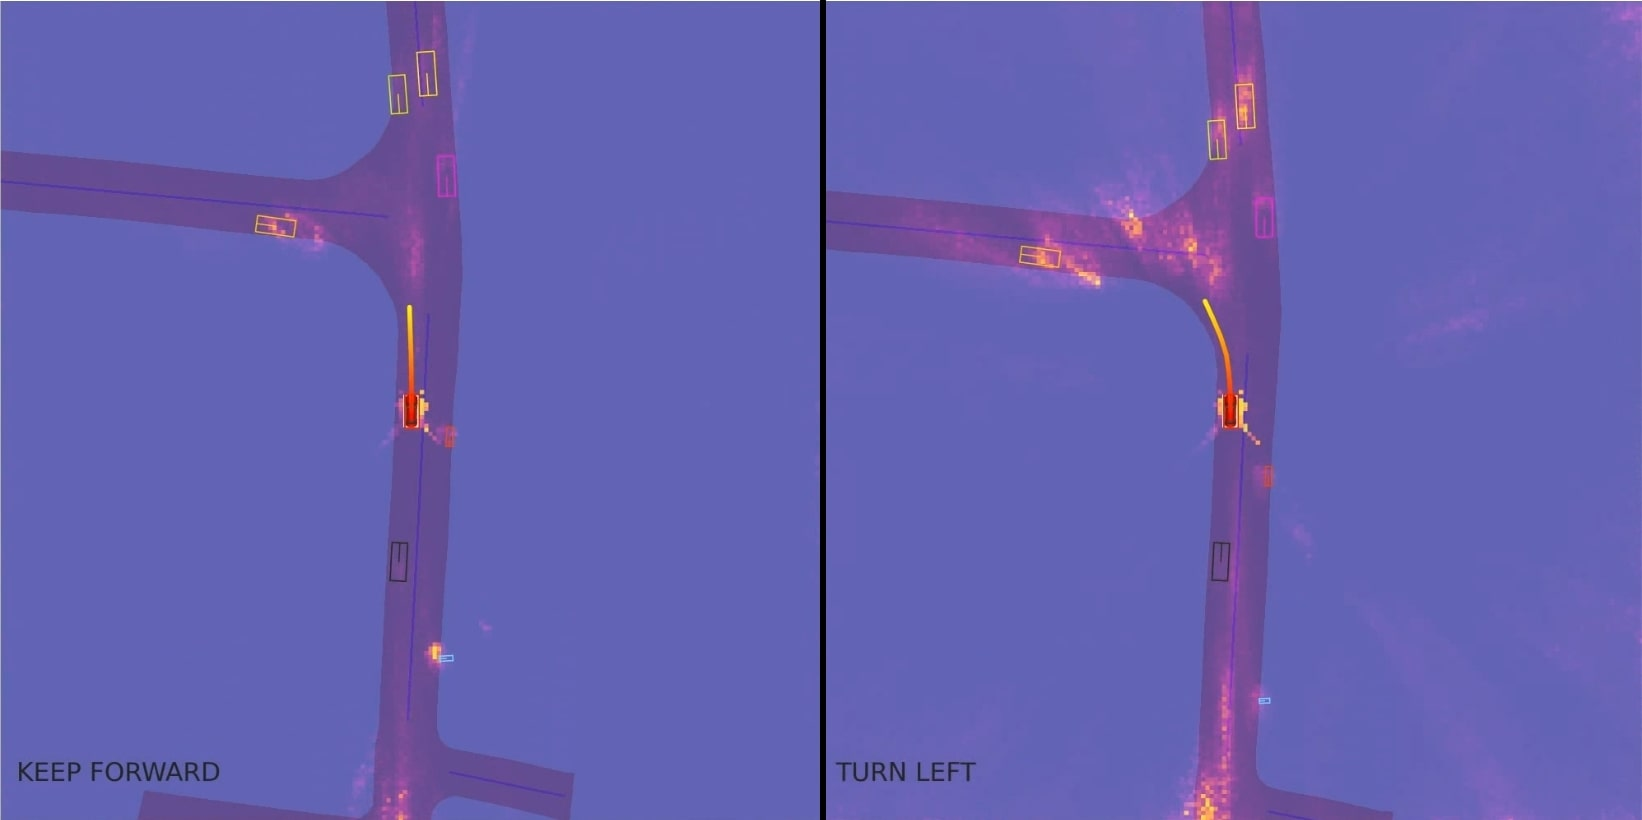
\includegraphics[width=0.6\linewidth]{UniAD/figures/vis_demo_small/vis-attn_mask.jpg}
  \caption{\textbf{导航指令效果与注意力掩码可视化.} 本文展示了如何根据导航指令关注不同区域。渲染了规划模块中BEV交互模块的注意力掩码、预测的跟踪边界框以及规划轨迹。导航指令显示在左下角，高精地图仅作为参考渲染展示。从左到右展示了同一时间序列中两个连续帧但具有不同导航指令的情况。可以观察到规划轨迹根据指令变化很大。同时，大量注意力集中在目标车道以及为自车让行的关键智能体上。}
  \label{fig:vis-supp-attn_mask}
\end{figure*}

\begin{figure*}[t!]
  \centering
  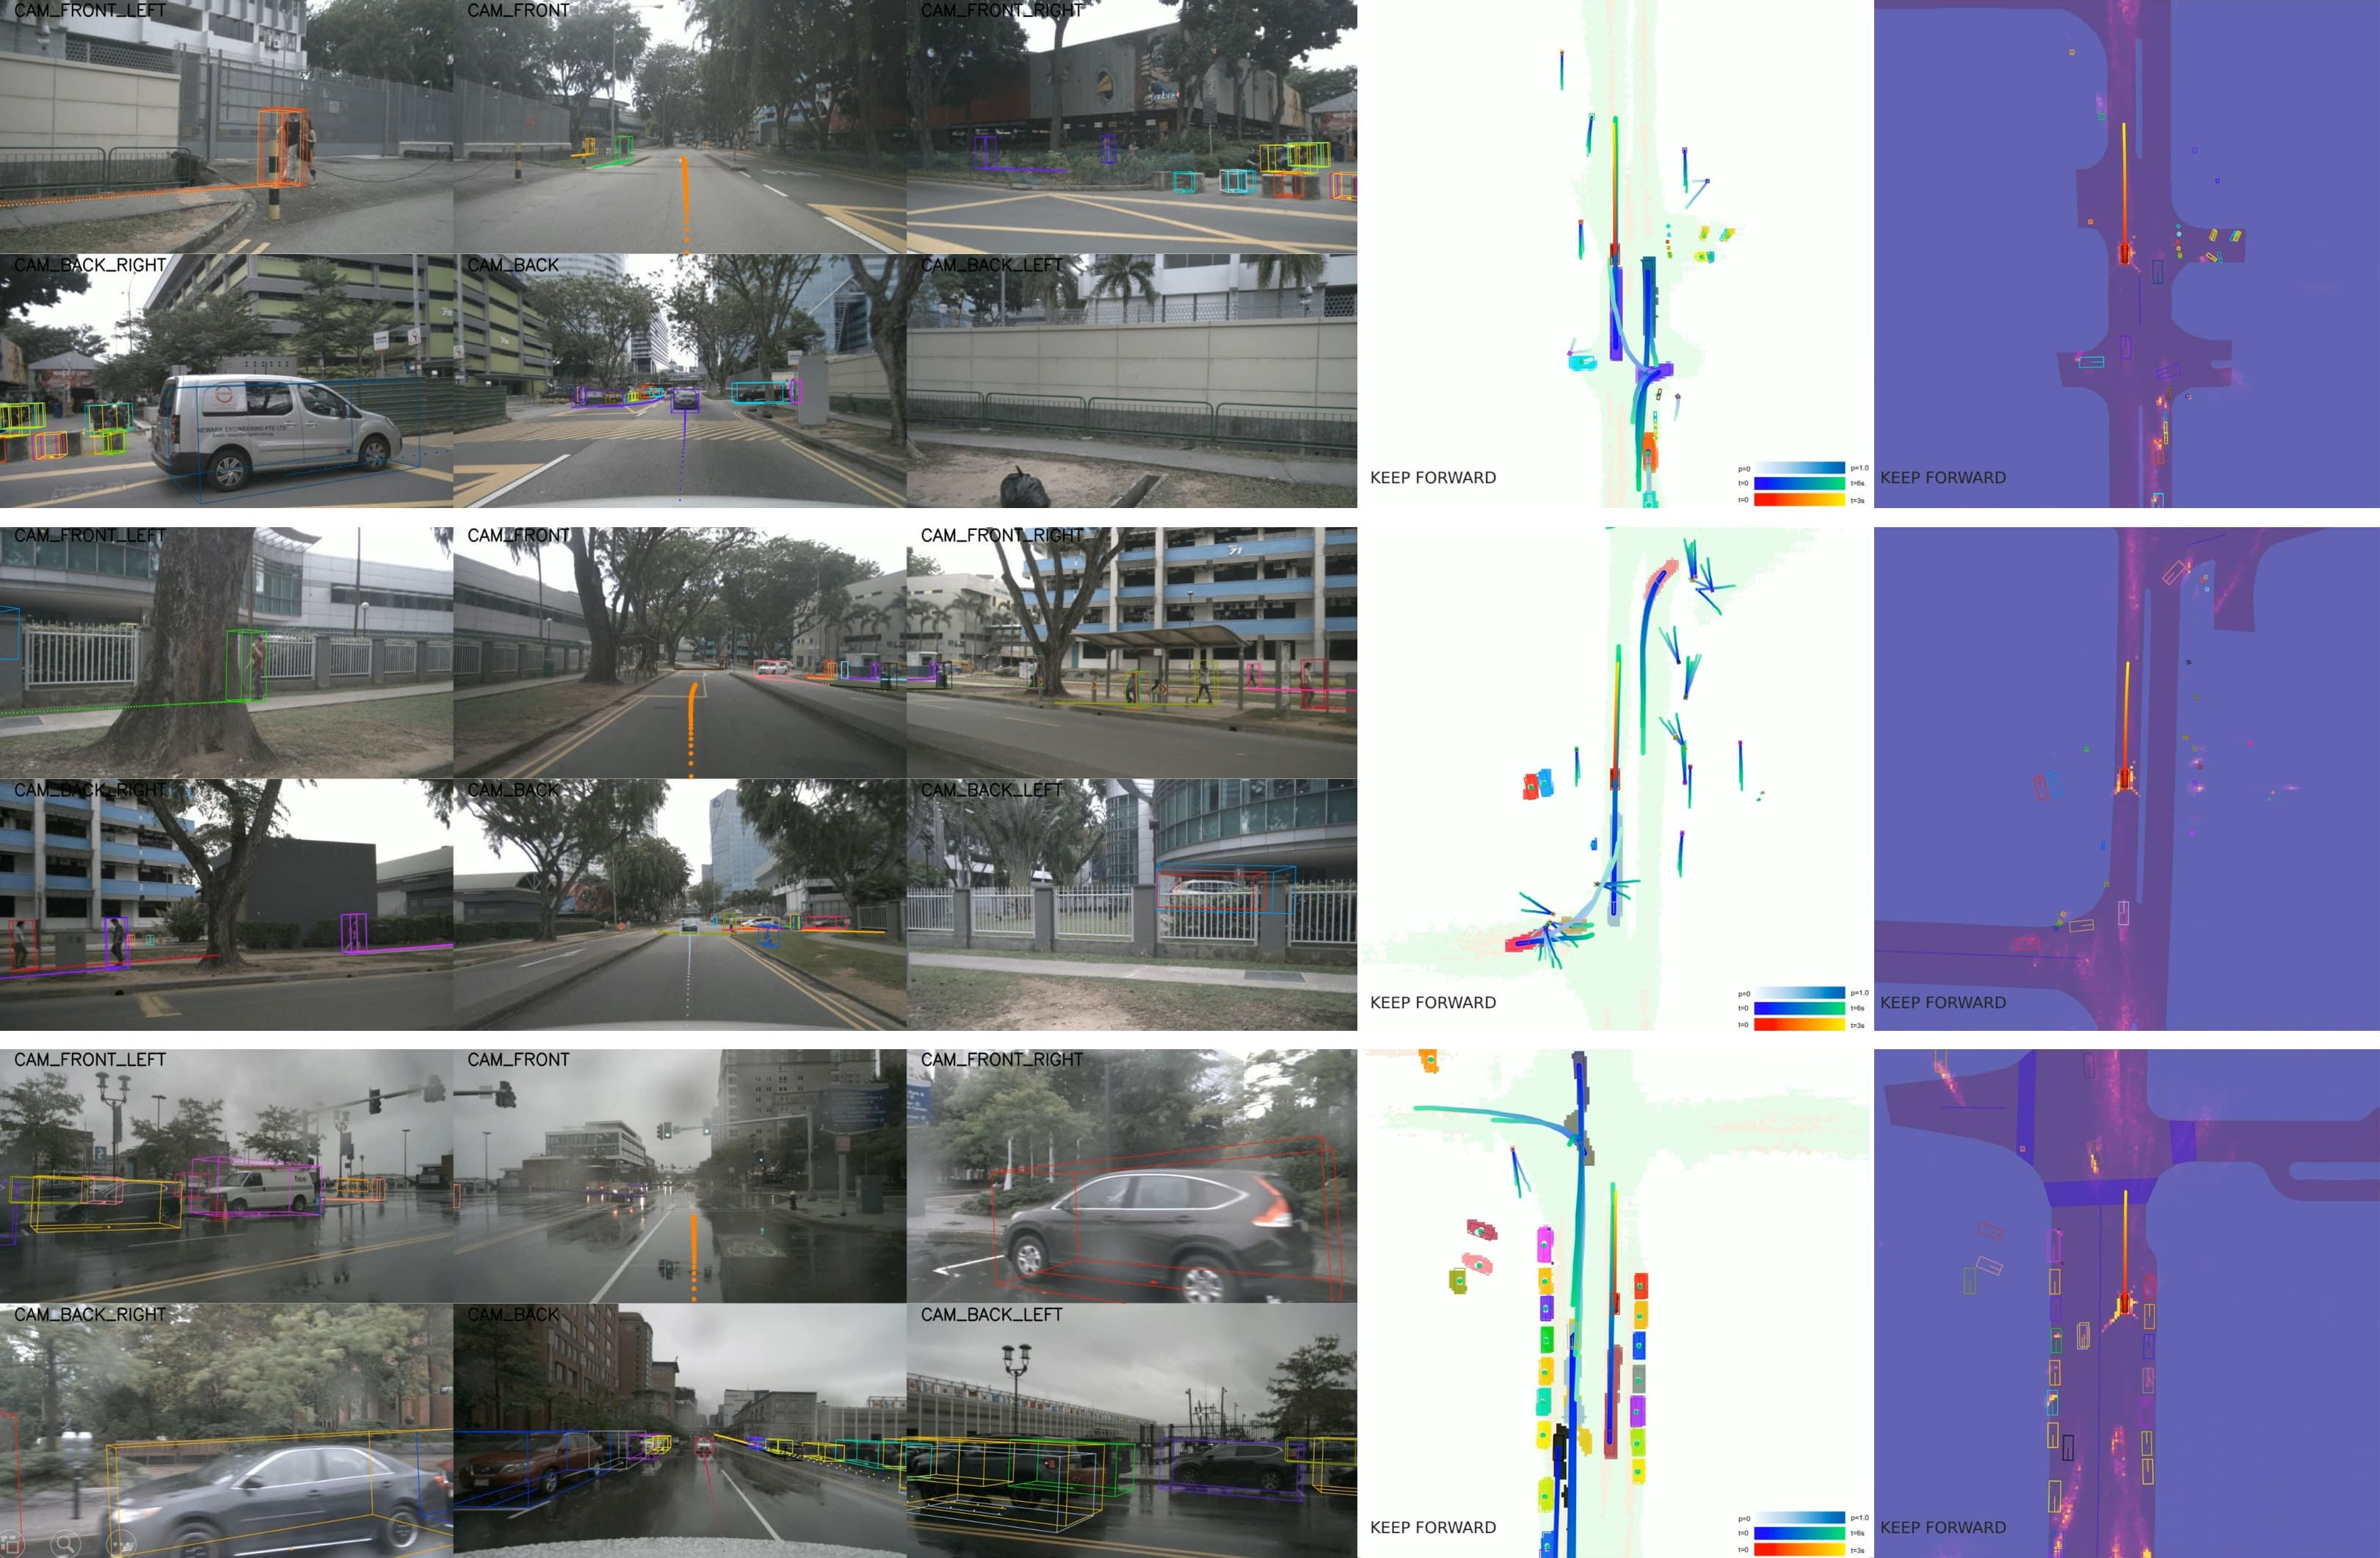
\includegraphics[width=0.98\textwidth]{UniAD/figures/vis_demo_small/vis-sota.jpg}
  \caption{\textbf{城市区域巡航可视化.} \\algname{}可以生成高质量且可解释的感知和预测结果，并做出安全驾驶操作。
  %
  前三列显示六个相机视角，最后两列分别是预测结果和规划模块的注意力掩码。每个智能体以不同颜色表示。仅选择运动预测中top-1和top-3的轨迹分别用于图像视图和BEV的可视化。}
  \label{fig:vis-supp-best}
\end{figure*}

\begin{figure*}[t!]
  \centering
  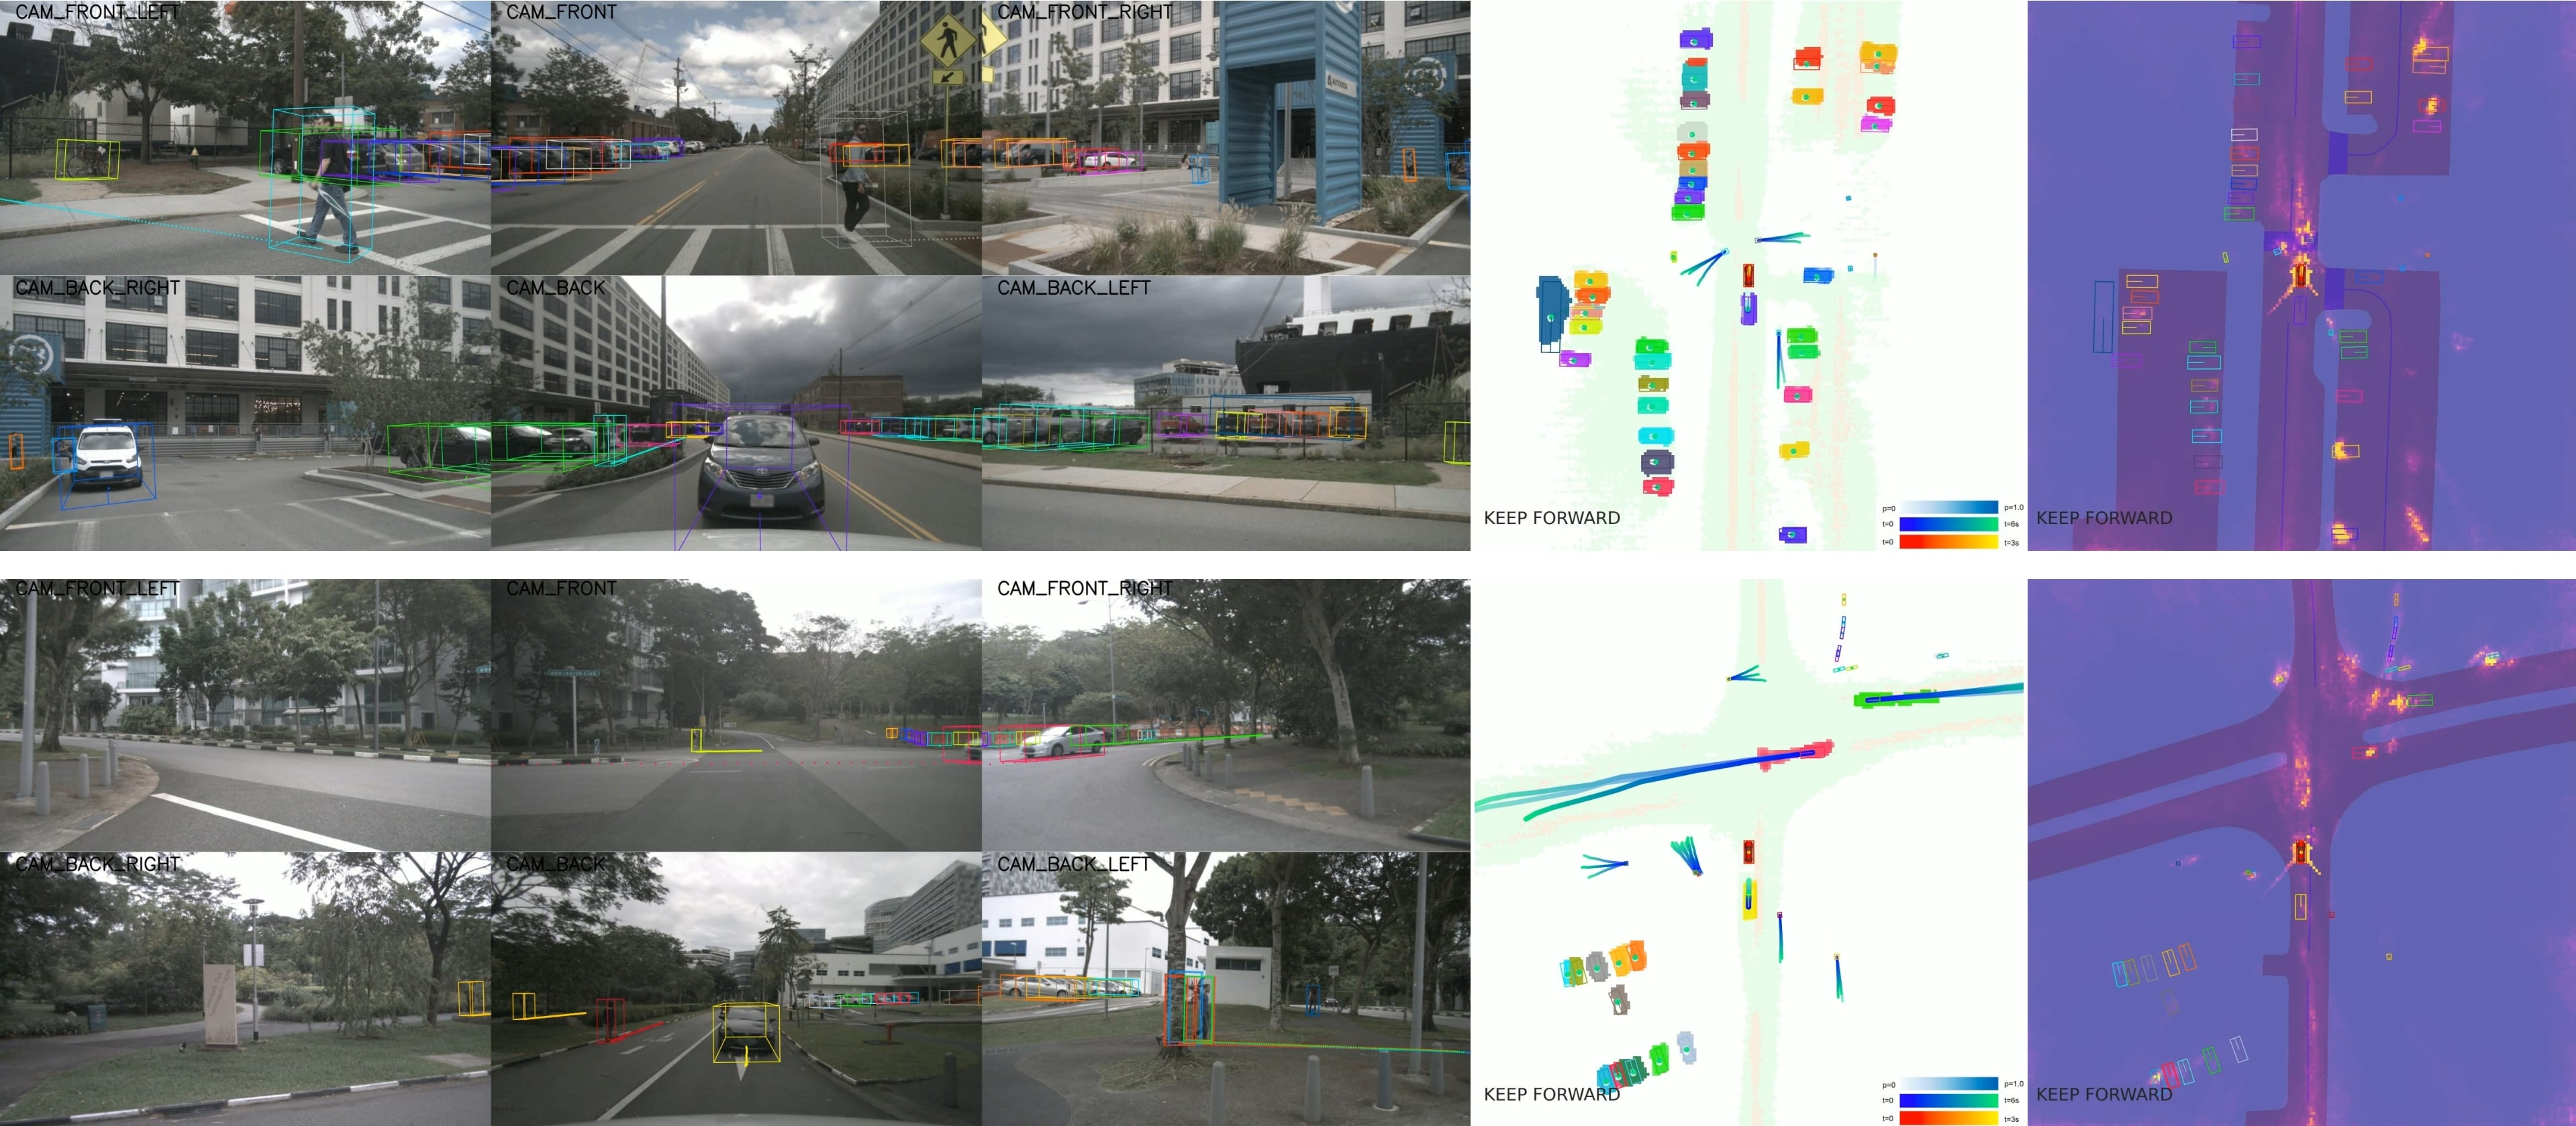
\includegraphics[width=0.98\textwidth]{UniAD/figures/vis_demo_small/vis-critical.jpg}
  \caption{\textbf{关键案例可视化.} 此处展示两个关键案例。第一个场景（上）显示自车正在避让两名过马路的行人，第二个场景（下）显示自车正在避让一辆快速行驶的车辆，并在十字路口附近等待无保护直行。可以观察到大量注意力集中在最关键的智能体（即行人和快速行驶车辆）以及预期目标位置上。}
  \label{fig:vis-supp-critical}
\end{figure*}


\begin{figure*}[t!]
  \centering
  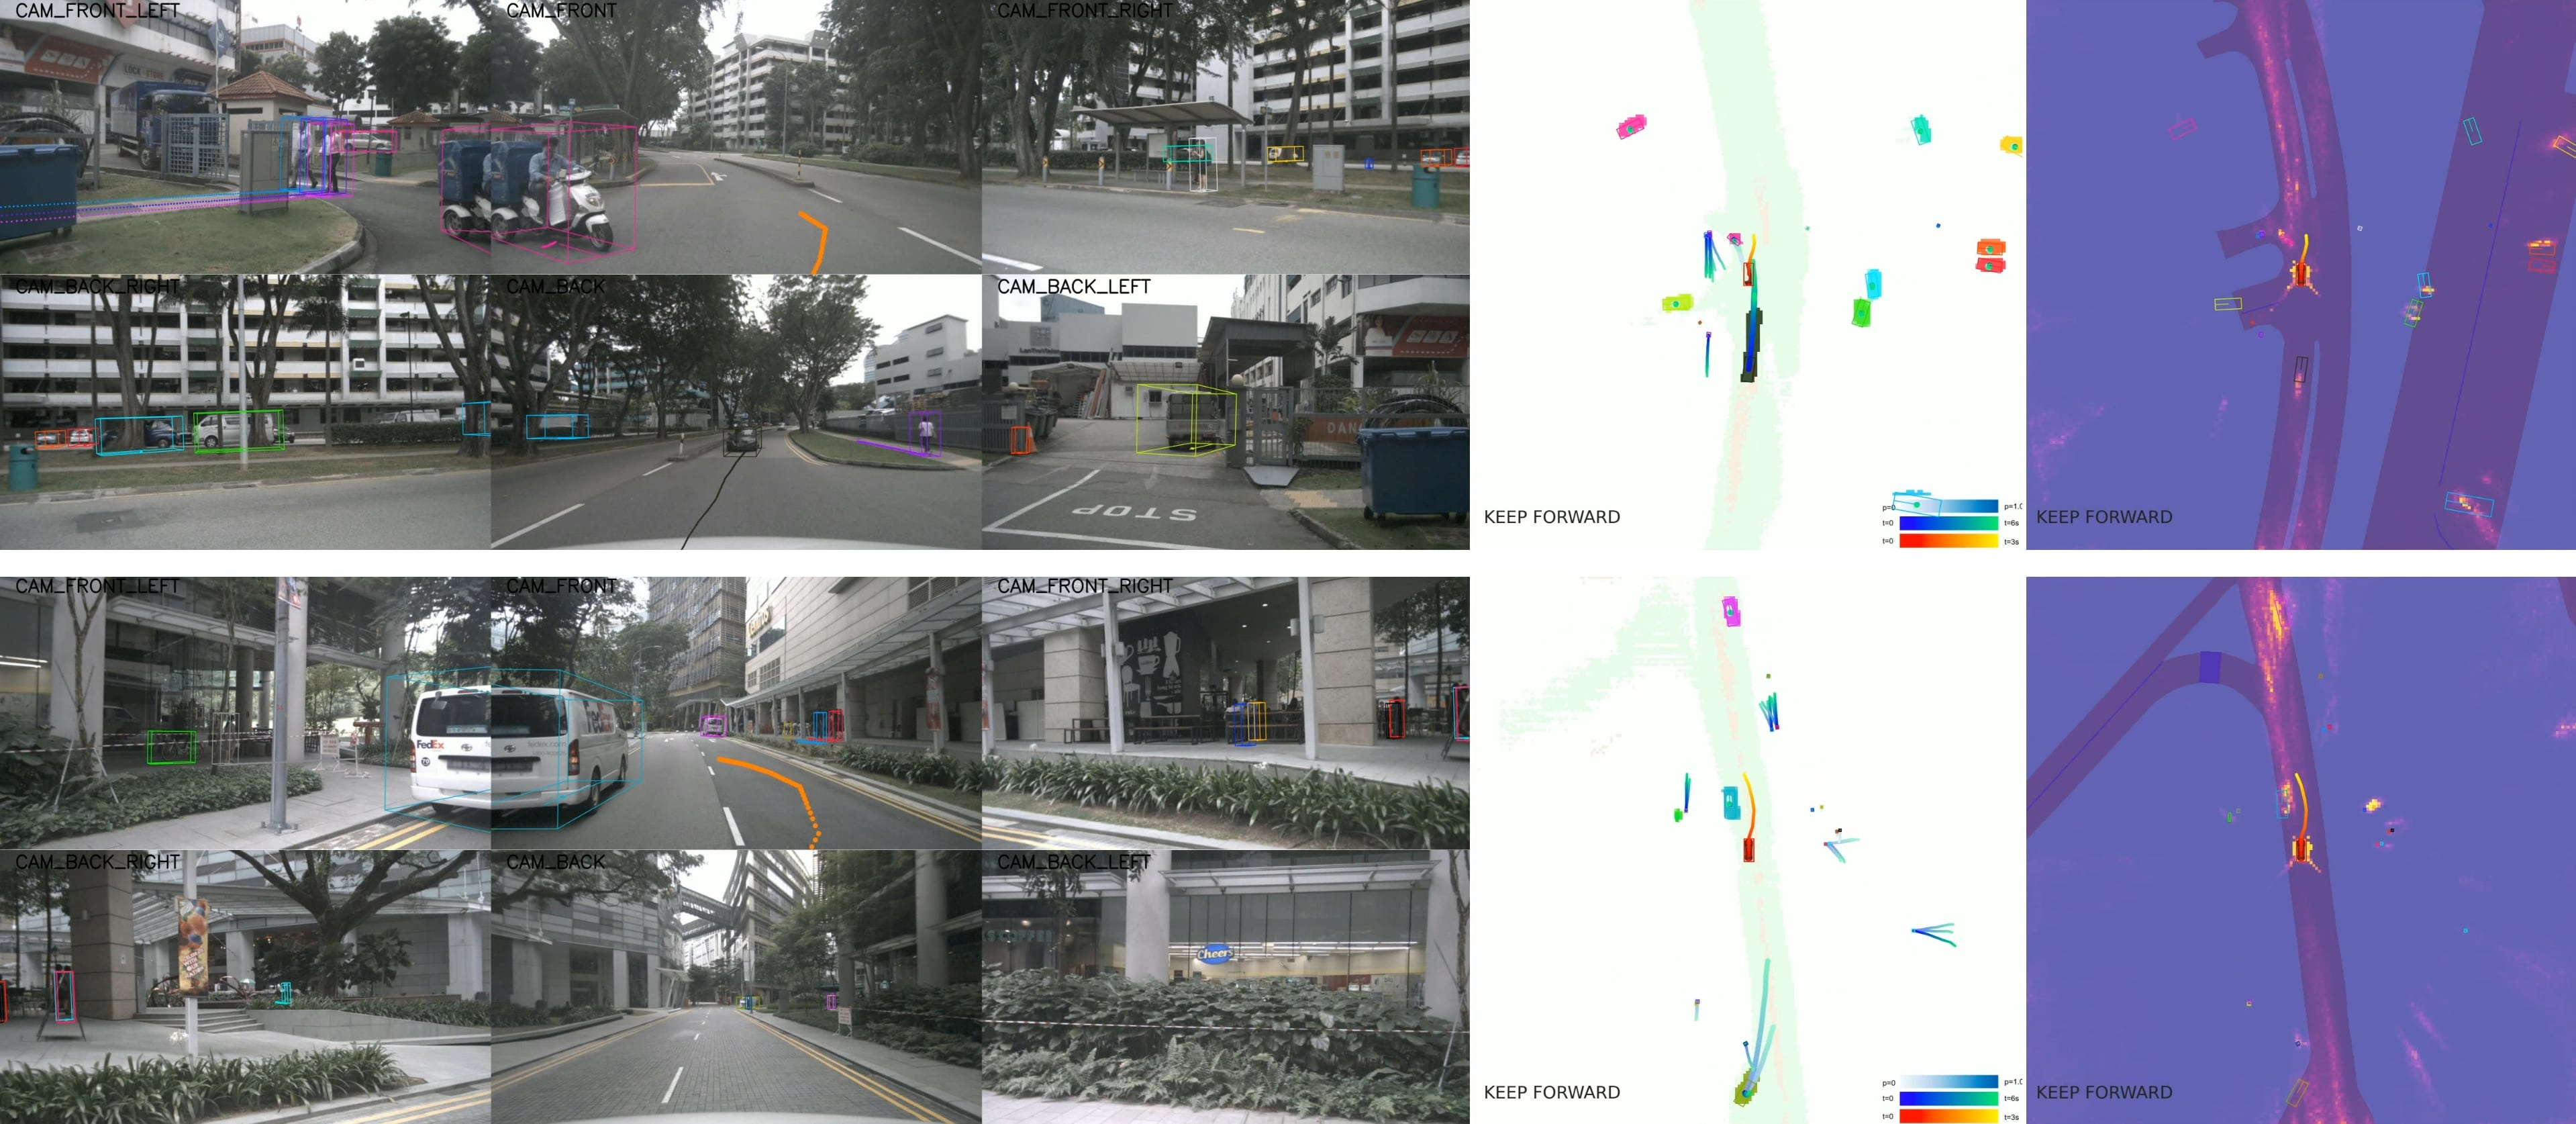
\includegraphics[width=\textwidth]{UniAD/figures/vis_demo_small/vis-col-avoid.jpg}
  \vspace{-12pt}
  \caption{\textbf{避障可视化.}
  %
  在这两个场景中，自车正在注意变道以避开障碍车辆。从注意力掩码可以观察到，本文方法关注障碍物以及前后方的道路。}
  \label{fig:vis-planning-obs-avoid}
\end{figure*}

\begin{figure*}[t!]
  \centering
  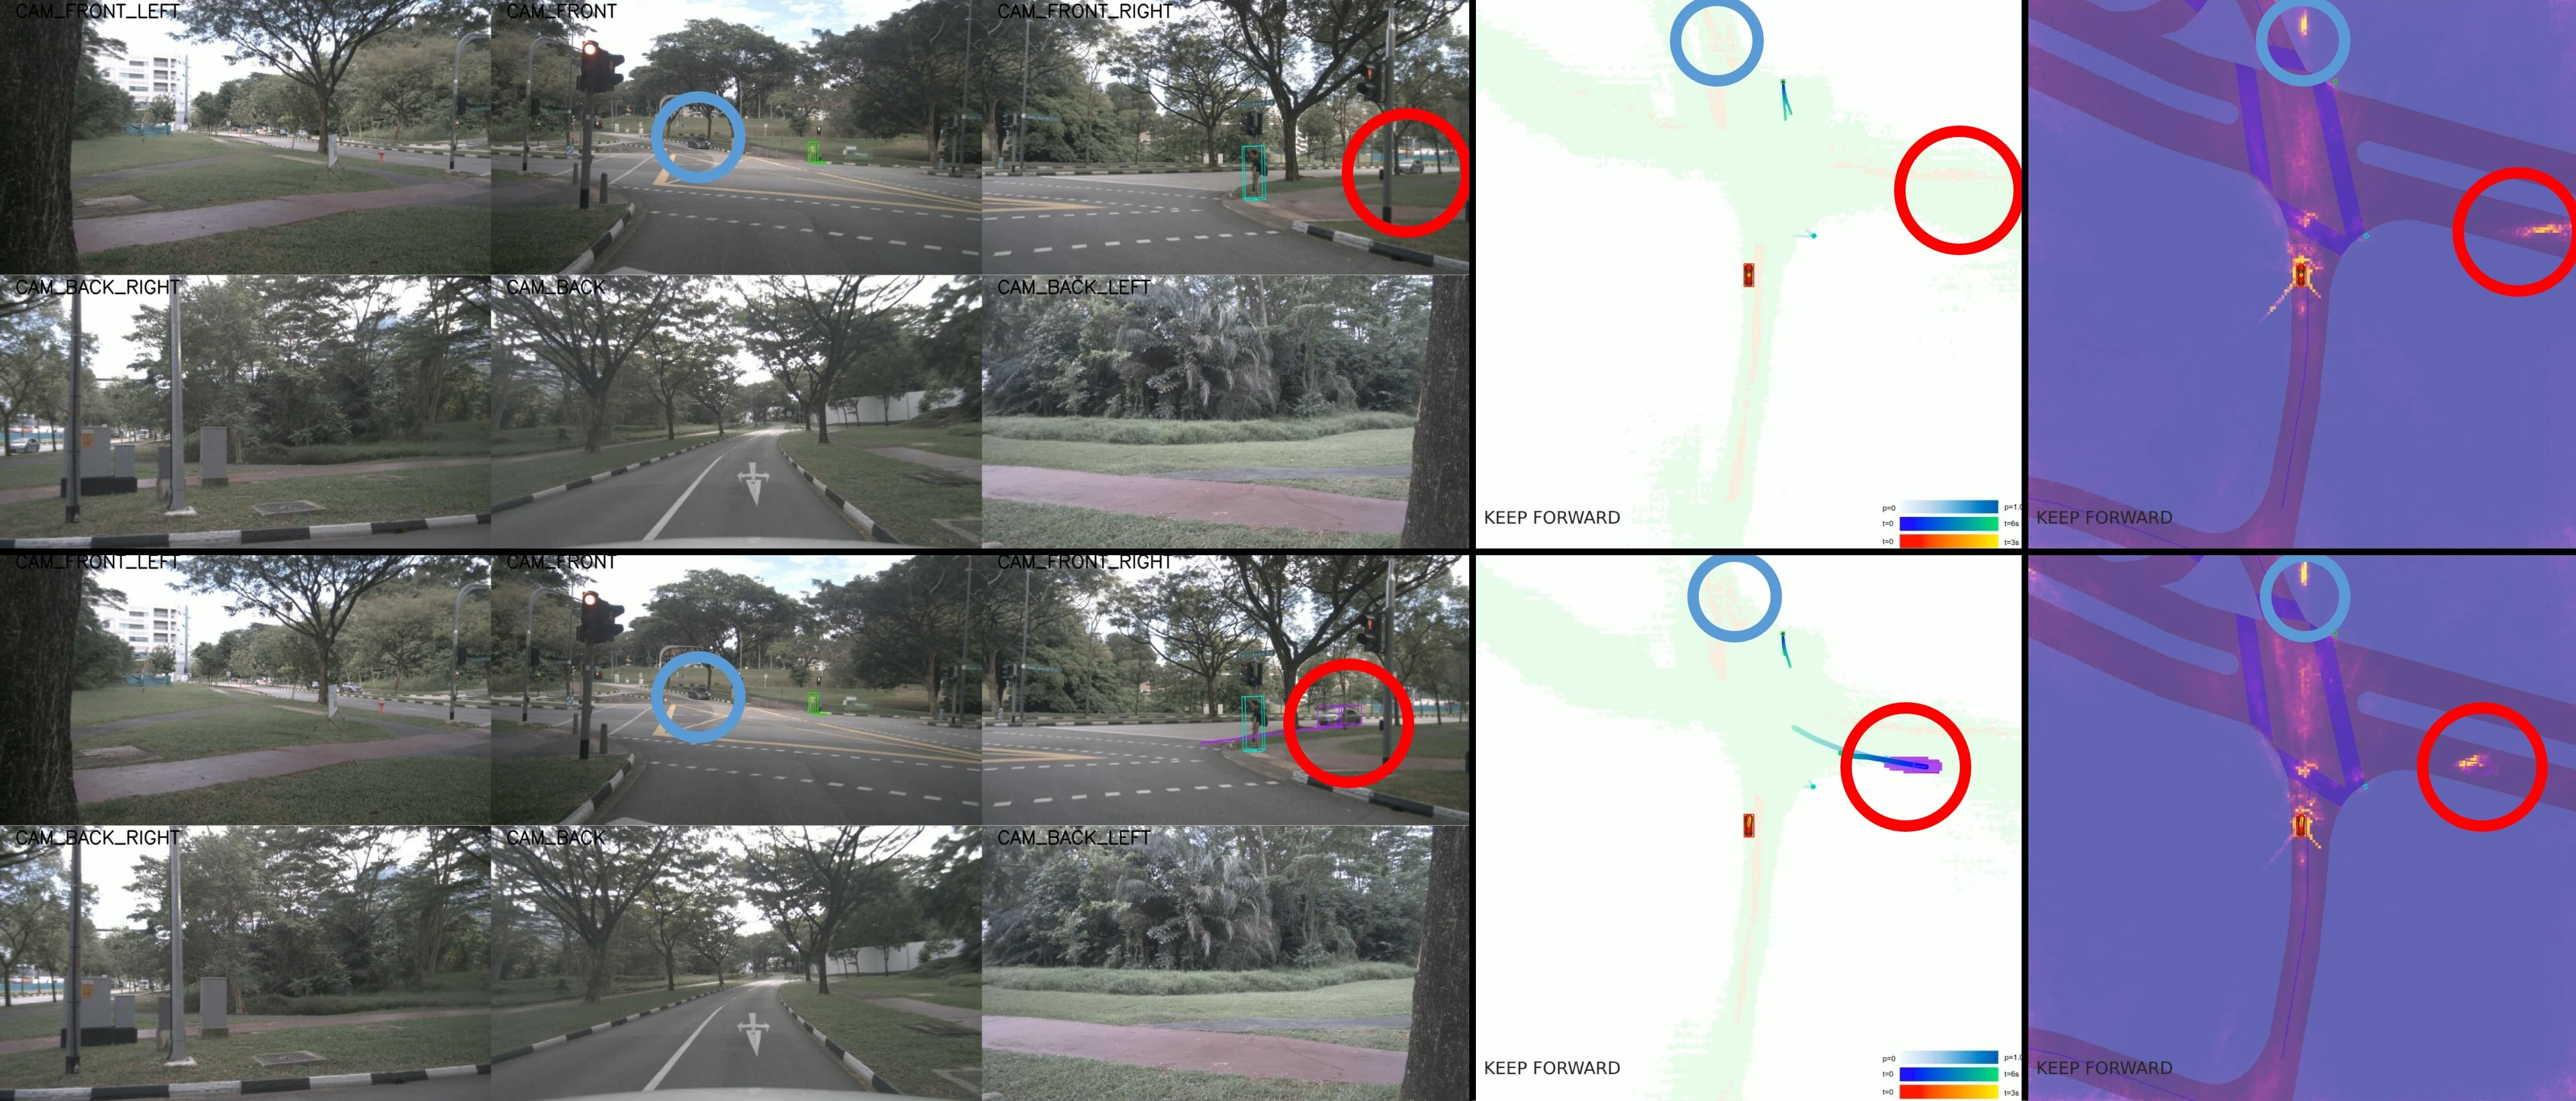
\includegraphics[width=\textwidth]{UniAD/figures/vis_demo_small/vis-failure1.jpg}
  \vspace{-12pt}
  \caption{\textbf{规划从感知失败中恢复的可视化.} 展示了一个有趣案例，前置模块出现不准确结果，但后续任务仍可恢复。上排和下排代表同一场景中的两个连续帧。
  %
  红色圆圈中的车辆从远处高速驶向十字路口。可以观察到跟踪模块起初遗漏了它，然后在后一帧捕获到。
  %
  蓝色圆圈显示一辆静止的汽车在让行，它在两帧中都被遗漏。有趣的是，即使在前置模块中被遗漏，这两辆车在规划器的注意力掩码中仍然有强烈响应。这意味着规划器仍然关注这些被遗漏但关键的目标，这在先前碎片化且非统一的驾驶系统中是难以实现的，展示了UniAD的鲁棒性。  }
  \label{fig:vis-supp-failure1}
\end{figure*}

\begin{figure*}[t!]
  \centering
  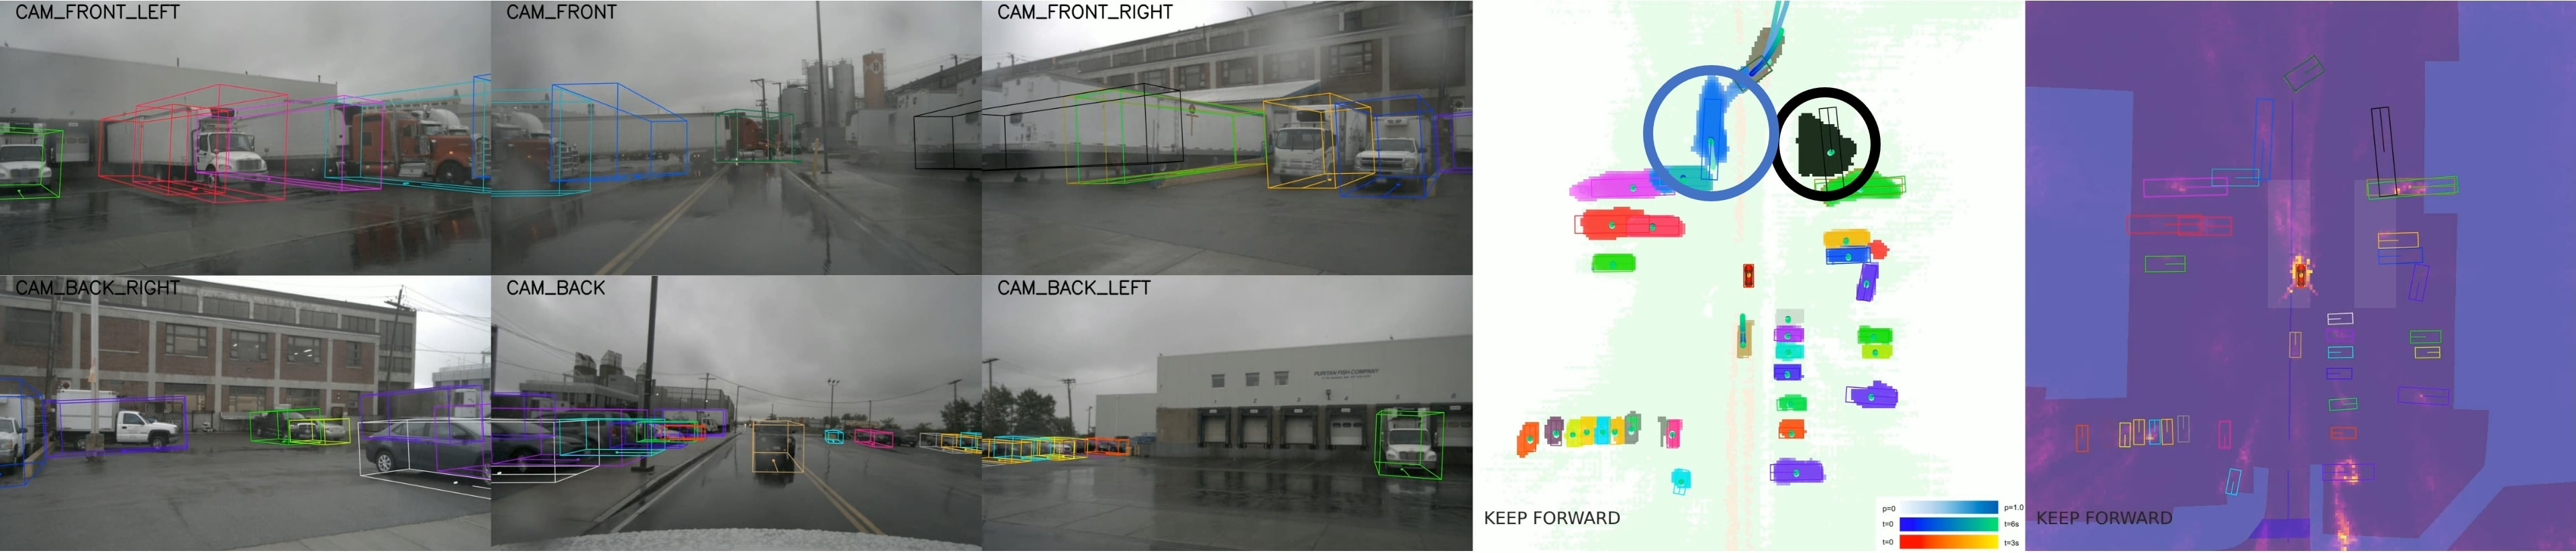
\includegraphics[width=\textwidth]{UniAD/figures/vis_demo_small/vis-failure2.jpg}
  \vspace{-12pt}
  \caption{\textbf{失败案例1.} 展示了一个长尾场景，带有白色集装箱的大型拖车占据了整条道路。可以观察到跟踪模块未能检测到前方拖车的准确尺寸和路边车辆的航向角。
  }
  \label{fig:vis-supp-failure2}
\end{figure*}

\begin{figure*}[t!]
  \centering
  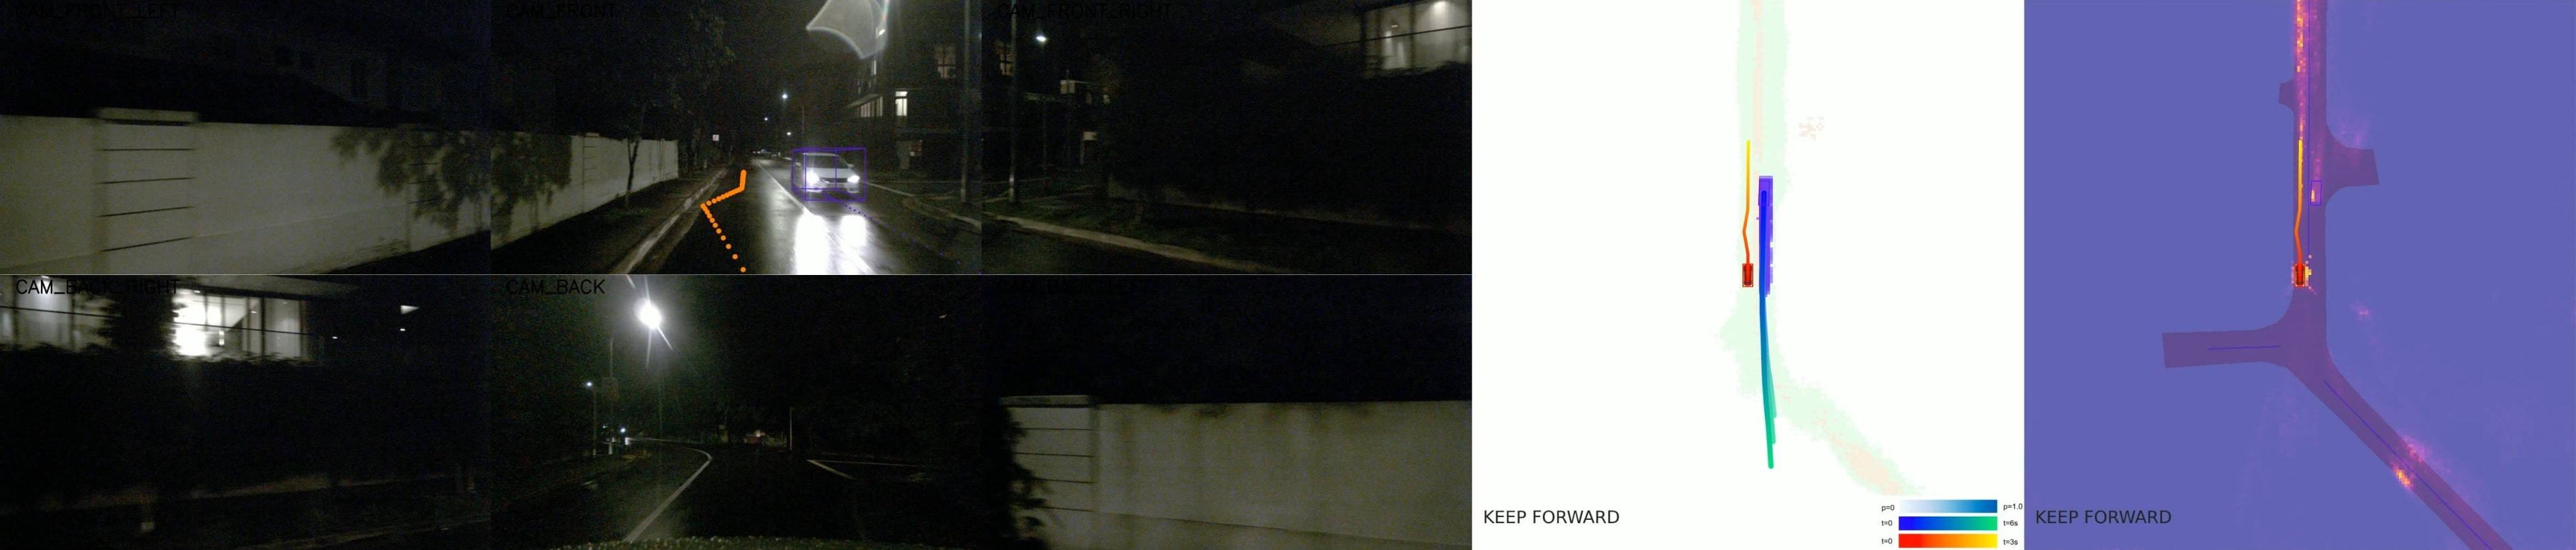
\includegraphics[width=\textwidth]{UniAD/figures/vis_demo_small/vis-failure3.jpg}
  \vspace{-12pt}
  \caption{\textbf{失败案例2.} 在此案例中，规划器对狭窄街道上的来车过度谨慎。黑暗环境是自动驾驶中长尾场景的关键类型之一。应用更小的碰撞损失权重和更多关于边界的约束可能缓解该问题。}
  \label{fig:vis-supp-failure3}
\end{figure*}

\end{document}
